\documentclass[oneside,a4paper,12pt]{book}

% ============================================================
% PACKAGES
% ============================================================
\usepackage[top=23.4mm, left=37mm, bottom=32mm, right=23.4mm]{geometry}
\usepackage{mathptmx}          % Times Roman font
\usepackage{setspace}           % Line spacing control
\onehalfspacing                 % 1.5 line spacing
\usepackage{fancyhdr}
\usepackage[hidelinks]{hyperref}
\usepackage{tikz}
\usetikzlibrary{arrows,arrows.meta,shapes,snakes,automata,backgrounds,petri,positioning,shapes.geometric,fit,calc,decorations.pathreplacing}
\usepackage{titlesec}
\usepackage{tabularx}
\usepackage[nottoc,notlot,notlof,numbib]{tocbibind}
\usepackage[titletoc]{appendix}
\usepackage{titletoc}
\usepackage{float}
\usepackage{subcaption}
\usepackage{multirow}
\usepackage{booktabs}
\usepackage{amsmath,amssymb}
\usepackage{listings}
\usepackage{enumitem}
\usepackage{algorithm}
\usepackage{algorithmic}
\usepackage{pgfgantt}
\usepackage{longtable}
\usepackage{ragged2e}

\renewcommand{\appendixname}{Annexure}
\renewcommand{\bibname}{References}
\setcounter{secnumdepth}{5}

% Listings style for code
\lstset{
  basicstyle=\footnotesize\ttfamily,
  breaklines=true,
  frame=single,
  numbers=left,
  numberstyle=\tiny,
  tabsize=2,
  captionpos=b,
  xleftmargin=2em,
  framexleftmargin=1.5em
}

% ============================================================
% PAGE STYLES
% ============================================================
\fancypagestyle{plain}{%
  \fancyhf{}
  \fancyfoot[C]{\fontsize{10}{12}\selectfont SCTR's PICT, Department of Computer Engineering 2025-26}
  \fancyfoot[R]{\thepage}
  \renewcommand{\headrulewidth}{0pt}
  \renewcommand{\footrulewidth}{1pt}
}

\fancypagestyle{frontmatter}{%
  \fancyhf{}
  \fancyfoot[C]{\fontsize{10}{12}\selectfont SCTR's PICT, Department of Computer Engineering 2025-26}
  \fancyfoot[R]{\thepage}
  \renewcommand{\headrulewidth}{0pt}
  \renewcommand{\footrulewidth}{1pt}
}

\fancypagestyle{mainmatter}{%
  \fancyhf{}
  \lhead{KiwiDB: LSM Tree Key-Value Store}
  \cfoot{\fontsize{10}{12}\selectfont SCTR's PICT, Department of Computer Engineering 2025-26}
  \rfoot{Page \thepage}
  \renewcommand{\headrulewidth}{2pt}
  \renewcommand{\footrulewidth}{1pt}
}

% ============================================================
% TITLE FORMATTING
% ============================================================
\titleformat{\chapter}[display]
{\fontsize{14}{17}\filcenter\bfseries}
{\vspace*{\fill}\MakeUppercase{\chaptertitlename}~\thechapter}
{1pc}
{\MakeUppercase}
[\thispagestyle{empty}\vspace*{\fill}\newpage]

\titleformat{\section}
{\fontsize{12}{15}\bfseries\raggedright}
{\thesection}{1em}{\MakeUppercase}

\titleformat{\subsection}
{\fontsize{12}{15}\bfseries\raggedright}
{\thesubsection}{1em}{}

\titleformat{\subsubsection}
{\fontsize{12}{15}\raggedright}
{\thesubsubsection}{1em}{}

\titlespacing*{\section}{0pt}{2\baselineskip}{1\baselineskip}
\titlespacing*{\subsection}{0pt}{1\baselineskip}{0.5\baselineskip}

% ============================================================
% BEGIN DOCUMENT
% ============================================================
\begin{document}

% ============================================================
% TITLE PAGE [P-1]
% ============================================================
\setlength{\parindent}{0mm}
\begin{center}
\vspace*{1\baselineskip}
{\bfseries \fontsize{12}{15} \selectfont A PROJECT REPORT ON \\}
\vspace*{1\baselineskip}
{\bfseries \fontsize{12}{15} \selectfont HIGH THROUGHPUT WRITE-OPTIMIZED KEY-VALUE STORE \\ USING LSM TREE ENGINE \\ \vspace*{2\baselineskip}}
{\fontsize{12}{15} \selectfont SUBMITTED TO THE SAVITRIBAI PHULE PUNE UNIVERSITY, PUNE
 \\ IN THE PARTIAL FULFILLMENT OF THE REQUIREMENTS \\ FOR THE AWARD OF THE DEGREE  \\
 \vspace*{1\baselineskip}
 OF \\
\vspace*{1\baselineskip}}
{\bfseries \fontsize{14}{17} \selectfont BACHELOR OF ENGINEERING (COMPUTER ENGINEERING) \\
\vspace*{1\baselineskip}}
{\bfseries \fontsize{12}{15} \selectfont SUBMITTED BY \\
\vspace*{1\baselineskip}}
Chaitanya Paraskar  \hspace{18mm}    Exam No:  B400050361 \\
Shreyash Dhas       \hspace{25.5mm}    Exam No:  B400050389 \\
Shreyash Gajbhiye   \hspace{19mm}    Exam No:  B400050407 \\
Shreyas Gopnarayan  \hspace{16mm}    Exam No:  B400050418 \\
\vspace*{1.5\baselineskip}


\includegraphics[width=100pt]{collegelogo.png} \\
\vskip 1cm
{\bfseries \fontsize{12}{15} \selectfont
DEPARTMENT OF COMPUTER ENGINEERING\\
PUNE INSTITUTE OF COMPUTER TECHNOLOGY \\
DHANKAWADI, PUNE 411043
\vspace*{1\baselineskip}

SAVITRIBAI PHULE PUNE UNIVERSITY\\
2025-2026
}
\end{center}

% ============================================================
% CERTIFICATE PAGE [P-2]
% ============================================================
\newpage
\begin{figure}[ht]
\centering

\includegraphics[width=100pt]{collegelogo.png}
\end{figure}

{\bfseries \fontsize{14}{17} \selectfont \centerline{CERTIFICATE}
\vspace*{0.5\baselineskip}}

\centerline{This is to certify that the project report entitled}
\vspace*{1\baselineskip}

{\bfseries \fontsize{12}{15} \selectfont \centerline{High Throughput Write-Optimised Key-Value Store}}
{\bfseries \fontsize{12}{15} \selectfont \centerline{using LSM Tree Engine}}
\vspace*{1\baselineskip}

\centerline{Submitted by}
\vspace*{0.5\baselineskip}
\begin{center}
Chaitanya Paraskar  \hspace{18mm}    Exam No:  B400050361 \\
Shreyash Dhas       \hspace{25.5mm}    Exam No:  B400050389 \\
Shreyash Gajbhiye   \hspace{19mm}    Exam No:  B400050407 \\
Shreyas Gopnarayan  \hspace{16mm}    Exam No:  B400050418 \\
\end{center}
\vspace*{1\baselineskip}

are bonafide students of this institute and the work has been carried out by them under the supervision of \textbf{Prof. M. V. Mane} and it is approved for the partial fulfillment of the requirement of \textbf{Savitribai Phule Pune University}, for the award of the degree of Bachelor of Engineering (Computer Engineering).

\vspace*{2\baselineskip}

\bgroup
\def\arraystretch{0.7}
\begin{tabular}{c c }
\textbf{Prof. M. V. Mane} &  \hspace{50 mm} \textbf{Dr. B. A. Sonkamble} \\
Internal Guide   &  \hspace{50 mm} Head \\
Dept. of Computer Engg.  &	\hspace{50 mm}Dept. of Computer Engg.  \\
\end{tabular}
%}
\begin{center}
%\fontsize{12}{18}\selectfont 
\vspace*{1\baselineskip}
{

\textbf{Dr. S. T. Gandhe}\\
Principal\\
Pune Institute of Computer Technology  
}
\end{center}
Place: Pune\\
Date:


% ============================================================
% ACKNOWLEDGEMENT
% ============================================================
\newpage
{\bfseries \fontsize{14}{17} \selectfont \centerline{ACKNOWLEDGEMENT}
\vspace*{2\baselineskip}}

\setlength{\parindent}{5em}

It gives us great pleasure in presenting the project report on \textbf{High Throughput Write-Optimised Key-Value Store using LSM Tree Engine}.

We would like to take this opportunity to thank our guide \textbf{Prof. M. V. Mane} for giving us all the help and guidance we needed. We are really grateful for her kind support and valuable suggestions throughout the development of this project.

We are also grateful to \textbf{Dr. B. A. Sonkamble}, Head of Computer Engineering Department, PICT, for his indispensable support and suggestions.

We express our sincere gratitude to the Principal, \textbf{Dr. S. T. Gandhe}, for providing us with the necessary infrastructure and resources. We also thank all faculty members and laboratory assistants of the Computer Engineering Department for their cooperation in the completion of this project.

\vspace*{3\baselineskip}
\begin{flushright}
Chaitanya Paraskar\\
Shreyash Dhas\\
Shreyash Gajbhiye\\
Shreyas Gopnarayan\\
(B.E. Computer Engineering)
\end{flushright}

% ============================================================
% ABSTRACT
% ============================================================
\newpage
{\bfseries \fontsize{14}{17} \selectfont \centerline{ABSTRACT}
\vspace*{2\baselineskip}}

\setlength{\parindent}{5em}

Traditional database storage engines built around B-trees are optimized for read-heavy workloads but suffer under intensive write operations due to random disk I/O. The Log-Structured Merge Tree (LSM tree) addresses this by converting random writes into sequential ones --- buffering data in memory and periodically flushing sorted batches to disk. This architecture underpins widely adopted systems such as LevelDB, RocksDB, and Cassandra.

This report presents KiwiDB, a prototype write-optimized key-value store built on the LSM tree architecture. The system implements the complete data lifecycle of an LSM-based engine: write-ahead logging for crash recovery, an in-memory memtable backed by a concurrent skip list, on-disk sorted string tables (SSTables) with bloom filters and sparse indexes, a parallel flush pipeline for memory-to-disk persistence, and a multi-level compaction engine for space reclamation and read performance maintenance. A hybrid compaction strategy --- tiering at Level 0 and leveling at subsequent levels --- reduces write amplification while keeping read costs bounded. The prototype also includes a web-based dashboard for real-time inspection of engine state across all stages of the data lifecycle.

The single-node storage engine presented here serves as a foundational building block for distributed key-value systems. Production systems such as etcd, TiKV, and CockroachDB are built by layering consensus protocols (Raft, Paxos) and distributed transaction logic on top of a local LSM-based storage engine. KiwiDB's modular architecture --- with well-defined interfaces between the WAL, memtable, SSTable, and compaction subsystems --- is designed to allow such extensions, providing a base upon which replication, sharding, and distributed coordination can be composed.

% ============================================================
% FRONT MATTER WITH ROMAN NUMERALS
% ============================================================
\frontmatter
\pagestyle{frontmatter}
\setlength{\parindent}{5em}

% --- Helper command for dot-leader entries ---
\newcommand{\tocentry}[2]{\noindent #1 \dotfill\ #2\\[4pt]}
\newcommand{\tocentrynum}[3]{\noindent #1\hspace{1.5em}#2 \dotfill\ #3\\[4pt]}

% --- List of Abbreviations ---
\newpage
\begin{center}
{\bfseries \fontsize{14}{17}\selectfont LIST OF ABBREVIATIONS}
\end{center}
\vspace*{2\baselineskip}

\renewcommand{\arraystretch}{1.3}
\noindent
\begin{tabularx}{\textwidth}{|p{4cm}|X|}
\hline
\textbf{Abbreviation} & \textbf{Illustration} \\
\hline
LSM & Log-Structured Merge Tree \\
\hline
KV & Key-Value \\
\hline
WAL & Write-Ahead Log \\
\hline
SSTable & Sorted String Table \\
\hline
GIL & Global Interpreter Lock \\
\hline
API & Application Programming Interface \\
\hline
REST & Representational State Transfer \\
\hline
MVCC & Multi-Version Concurrency Control \\
\hline
CRC & Cyclic Redundancy Check \\
\hline
FPR & False Positive Rate \\
\hline
LRU & Least Recently Used \\
\hline
SPA & Single Page Application \\
\hline
FIFO & First In, First Out \\
\hline
ASGI & Asynchronous Server Gateway Interface \\
\hline
ABC & Abstract Base Class \\
\hline
DFD & Data Flow Diagram \\
\hline
UML & Unified Modeling Language \\
\hline
SDLC & Software Development Life Cycle \\
\hline
mmap & Memory-Mapped I/O \\
\hline
\end{tabularx}

% --- List of Figures ---
\newpage
\begin{center}
{\bfseries \fontsize{14}{17}\selectfont LIST OF FIGURES}
\end{center}
\vspace*{2\baselineskip}

\renewcommand{\arraystretch}{1.3}
\noindent
\begin{tabularx}{\textwidth}{|p{2cm}|X|p{1.5cm}|}
\hline
\textbf{Figure} & \textbf{Illustration} & \textbf{Page No.} \\
\hline
4.1 & KiwiDB Layered Architecture & \pageref{fig:arch} \\
\hline
4.2 & DFD Level 0 --- Context Diagram & \pageref{fig:dfd0} \\
\hline
4.3 & DFD Level 1 --- Major Subsystems and Data Stores & \pageref{fig:dfd1} \\
\hline
4.4 & DFD Level 2 --- Write Path Detail & \pageref{fig:dfd2} \\
\hline
4.5 & Use Case Diagram for KiwiDB & \pageref{fig:usecase} \\
\hline
4.6 & Activity Diagram --- Write Path & \pageref{fig:activity} \\
\hline
4.7 & Sequence Diagram --- Put, Get, and Flush Operations & \pageref{fig:sequence} \\
\hline
4.8 & Class Diagram --- Core Class Hierarchy & \pageref{fig:classdiag} \\
\hline
4.9 & Component Diagram & \pageref{fig:component} \\
\hline
4.10 & Deployment Diagram & \pageref{fig:deploy} \\
\hline
4.11 & State Machine Diagram --- SSTableWriter Lifecycle & \pageref{fig:statemachine} \\
\hline
5.1 & Project Timeline (Gantt Chart) & \pageref{fig:gantt} \\
\hline
6.1 & Parallel Flush Pipeline with Event-Chain Ordering & \pageref{fig:flush-pipeline} \\
\hline
\end{tabularx}

% --- List of Tables ---
\newpage
\begin{center}
{\bfseries \fontsize{14}{17}\selectfont LIST OF TABLES}
\end{center}
\vspace*{2\baselineskip}

\renewcommand{\arraystretch}{1.3}
\noindent
\begin{tabularx}{\textwidth}{|p{2cm}|X|p{1.5cm}|}
\hline
\textbf{Table} & \textbf{Illustration} & \textbf{Page No.} \\
% \hline
% 2.1 & Comparative Summary of Reviewed Systems and KiwiDB & \pageref{tab:lit-summary} \\
\hline
4.1 & Thread and Async Model for Each Engine Component & \pageref{tab:thread-model} \\
\hline
4.2 & Write Amplification Comparison & \pageref{tab:write-amp} \\
\hline
6.1 & Project Modules Overview & \pageref{tab:modules} \\
\hline
7.1 & Representative Test Cases and Results & \pageref{tab:testcases} \\
\hline
\end{tabularx}

% Override chapter format for TOC so title and content appear on same page
{
\titleformat{\chapter}
{\fontsize{14}{17}\filcenter\bfseries}
{}
{0pt}
{\MakeUppercase}
\titlespacing*{\chapter}{0pt}{0pt}{2\baselineskip}
\tableofcontents
}

% ============================================================
% MAIN MATTER — Arabic page numbers starting from 1
% ============================================================
\mainmatter
\pagestyle{mainmatter}
\setlength{\parindent}{5em}

% %%%%%%%%%%%%%%%%%%%%%%%%%%%%%%%%%%%%%%%%%%%%%%%%%%%%%%%%%%%%
% CHAPTER 1: INTRODUCTION
% %%%%%%%%%%%%%%%%%%%%%%%%%%%%%%%%%%%%%%%%%%%%%%%%%%%%%%%%%%%%
\chapter{Introduction}

\section{Overview}

With the rapid growth of web applications and cloud computing, key-value (KV) stores have become a critical component of modern data infrastructure. A KV store maps a set of keys to associated values and can be considered a simplified interface over more complex storage systems. Without having to provide features usually required for a relational database system, KV stores offer higher performance, better scalability, and greater availability \cite{c1}. They play a central role in data centers supporting Internet-scale services, including BigTable \cite{c2} at Google, Cassandra \cite{c3} at Facebook, and Dynamo \cite{c4} at Amazon.

The B+ tree is a common structure used in traditional databases because its high fanout reduces the number of I/O operations for a query. However, it is highly inefficient for random insertions and updates. When there are intensive mutations, B+ trees lead to a large number of costly disk seeks and significantly degraded performance. The Log-Structured Merge Tree (LSM tree) \cite{c5} addresses this by transforming random writes into sequential writes: incoming data is sorted in an in-memory buffer and flushed to storage as a whole when the buffer is full. Many popular KV stores adopt this design, including BigTable \cite{c2}, Cassandra \cite{c3}, HBase \cite{c6}, and LevelDB \cite{c7}.

This project presents \textbf{KiwiDB}, a complete LSM tree key-value store implemented from scratch in Python 3.12+. The system comprises approximately 6,600 lines of type-checked Python code across 25 modules, with 211 automated tests, an async-native API, and a built-in web dashboard for real-time engine inspection.

\section{Motivation}

Despite the maturity of existing LSM-based systems, we observe two limitations that motivate this work:

\textbf{Synchronous APIs.} LevelDB and RocksDB \cite{c8} expose blocking C++ interfaces. Modern Python applications built with frameworks like FastAPI and aiohttp run on \texttt{asyncio} event loops. Integrating a synchronous storage engine requires thread-pool wrappers that add latency, complexity, and concurrency bugs. To the best of our knowledge, no existing LSM implementation offers a natively asynchronous API.

\textbf{Opaque Internals.} Production engines prioritize throughput over observability. Inspecting memtable state, bloom filter hit rates, compaction progress, or SSTable layouts requires external tooling. Internal design decisions are documented sparsely, making these systems difficult to learn from.

Additionally, from an academic perspective, building a storage engine from first principles provides deep insight into database internals --- write-ahead logging, memory management, disk persistence, concurrency control, and background job scheduling --- topics that are typically studied only theoretically.

\section{Problem Definition and Objectives}

\textbf{Problem Statement:} Design and implement a write-optimized key-value store that provides an async-native API, crash-safe persistence, background compaction with GIL bypass, and full observability via a web dashboard.

\textbf{Objectives:}
\begin{enumerate}[leftmargin=2em]
    \item Implement an \textbf{async-native API} where all public operations (\texttt{put}, \texttt{get}, \texttt{delete}, \texttt{flush}, \texttt{close}) are async coroutines that never block the event loop.
    \item Implement a \textbf{write-ahead log} with CRC32 integrity verification for crash recovery.
    \item Design a \textbf{concurrent skip list} memtable with fine-grained per-node locking for writes and lock-free reads.
    \item Implement \textbf{SSTable persistence} with bloom filters, sparse indexes, and memory-mapped reads.
    \item Design a \textbf{parallel flush pipeline} with event-chain ordered commits for concurrent SSTable writes.
    \item Implement \textbf{subprocess-based compaction} via \texttt{ProcessPoolExecutor} to bypass CPython's GIL for true CPU parallelism.
    \item Build a \textbf{web dashboard} with FastAPI backend and React frontend for real-time engine inspection.
\end{enumerate}

\section{Project Scope and Limitations}

\textbf{Scope:} KiwiDB is a single-node, embedded key-value store supporting point reads and writes with crash safety. It includes a REPL interface, REST API, and web dashboard. It is designed as both a functional storage engine and an educational tool.

\textbf{Limitations:}
\begin{itemize}[leftmargin=2em]
    \item No range query support (although the internal merge iterator could be extended).
    \item No block compression (LZ4/zstd).
    \item No multi-key transactions or batch writes.
    \item Single-node only; no replication or distributed operation.
    \item 10--100$\times$ lower raw throughput compared to C++ implementations due to Python's interpreted nature.
\end{itemize}

\section{Methodologies of Problem Solving}

The project follows an \textbf{iterative and incremental} development methodology. Each subsystem (WAL, memtable, SSTable, compaction, flush pipeline) was designed, implemented, and tested independently before being integrated into the engine coordinator. Key methodological practices include:

\begin{itemize}[leftmargin=2em]
    \item \textbf{Test-driven development:} 211+ automated tests written alongside implementation using pytest and pytest-asyncio.
    \item \textbf{Formal type checking:} Dual static analysis with mypy (strict mode) and basedpyright (strict mode) to catch type errors at compile time.
    \item \textbf{Design from first principles:} Architecture informed by academic literature on LSM trees, with innovations tailored to Python's runtime model.
    \item \textbf{Security analysis:} bandit static security scanner run on every change.
    \item \textbf{Continuous documentation:} Design documents and API reference maintained alongside code using MkDocs.
\end{itemize}

% %%%%%%%%%%%%%%%%%%%%%%%%%%%%%%%%%%%%%%%%%%%%%%%%%%%%%%%%%%%%
% CHAPTER 2: LITERATURE SURVEY
% %%%%%%%%%%%%%%%%%%%%%%%%%%%%%%%%%%%%%%%%%%%%%%%%%%%%%%%%%%%%
\chapter{Literature Survey}

This chapter reviews the foundational literature and existing systems that inform the design of KiwiDB.

\vspace{1\baselineskip}

\textbf{1. O'Neil et al. --- The Log-Structured Merge Tree (1996) \cite{c5}}

O'Neil et al. proposed the LSM tree as a write-optimized alternative to B-trees. The key insight is to buffer incoming writes in an in-memory component and periodically flush sorted runs to disk. On-disk components are merged in the background to reclaim space and maintain read performance. This design transforms random writes into sequential I/O, which is significantly faster on both HDDs and SSDs. The LSM tree forms the foundation of KiwiDB's architecture.

\vspace{1\baselineskip}

\textbf{2. Google --- LevelDB (2011) \cite{c7}}

LevelDB is the canonical open-source LSM implementation, originating from Google's BigTable. It uses a skip list as the in-memory memtable, write-ahead logging for durability, and a multi-level compaction strategy where each level has non-overlapping key ranges. LevelDB serves as KiwiDB's primary baseline for comparison. However, LevelDB has two limitations: a single background thread for both flush and compaction, and a fully synchronous API. KiwiDB addresses both.

\vspace{1\baselineskip}

\textbf{3. Facebook --- RocksDB (2013) \cite{c8}}

RocksDB extends LevelDB with concurrent compaction, column families, configurable compaction strategies, and a lock-free skip list using compare-and-swap (CAS) atomics. It remains the most widely deployed LSM engine. KiwiDB borrows the concept of multiple immutable memtables from RocksDB but adopts a different concurrency model suited to Python's GIL.

\vspace{1\baselineskip}

\textbf{4. Wang et al. --- LOCS: LSM on Open-Channel SSD (2014) \cite{c9}}

Wang et al. extended LevelDB to exploit channel-level parallelism of open-channel SSDs by increasing the number of immutable memtables and flushing them concurrently to separate SSD channels. Their work demonstrated up to 4$\times$ throughput improvement. KiwiDB shares the insight that concurrent flush improves throughput but achieves it at the software level with an event-chain commit mechanism on commodity storage.

\vspace{1\baselineskip}

\textbf{5. Dayan et al. --- Monkey: Optimal Navigable KV Store (2017) \cite{c10}}

Monkey optimizes bloom filter memory allocation across LSM levels. By assigning more bits to lower levels (where reads are more frequent), Monkey minimizes the expected number of false positive I/Os. KiwiDB takes a different approach: instead of cross-level optimization, each bloom filter is sized optimally using the \emph{actual record count} at write time, producing right-sized filters without global tuning.

\vspace{1\baselineskip}

\textbf{6. Dayan and Idreos --- Dostoevsky (2018) \cite{c11}}

Dostoevsky introduces ``lazy leveling'' as a hybrid between tiering and leveling. The largest level uses tiering (cheaper writes) while smaller levels use leveling (cheaper reads). KiwiDB's L0-tiering / L1-leveling strategy achieves a similar write amplification reduction through a simpler design: L0 files are unsorted (tiered), while L1+ levels maintain a single merged file each.

\vspace{1\baselineskip}

\textbf{7. Luo and Carey --- LSM-based Storage Techniques: A Survey (2020) \cite{c12}}

This comprehensive survey formalizes the LSM design space across four dimensions: merge policy (tiering vs.\ leveling), size ratio, merge trigger, and component organization. It provides the theoretical framework within which KiwiDB's hybrid strategy can be analyzed. The survey also identifies write amplification as the primary bottleneck in leveled compaction --- exactly what KiwiDB's L0 tiering addresses.

\vspace{1\baselineskip}

\textbf{8. Bloom --- Space/Time Trade-offs in Hash Coding (1970) \cite{c13}}

Bloom proposed the probabilistic data structure now known as the bloom filter. It allows membership testing with no false negatives and a tunable false positive rate. Each SSTable in KiwiDB includes a bloom filter that eliminates unnecessary disk reads during point lookups. KiwiDB uses MurmurHash3 with seed variations as the hash function family.

\vspace{1\baselineskip}

\textbf{9. Herlihy et al. --- A Provably Correct Concurrent Skip List (2006) \cite{c14}}

Herlihy et al. presented a concurrent skip list algorithm with fine-grained locking for writers and lock-free traversal for readers. KiwiDB's skip list implementation is adapted from this design, with per-node locks for writers and GIL-atomic boolean flag checks for lock-free readers --- a simplification made possible by CPython's GIL guaranteeing atomic attribute reads.

\vspace{1\baselineskip}

\textbf{10. Lakshman and Malik --- Cassandra (2010) \cite{c3}}

Cassandra is a distributed LSM-based storage system designed for high availability and partition tolerance. While KiwiDB is single-node, Cassandra's write path (commit log $\rightarrow$ memtable $\rightarrow$ SSTable) informed KiwiDB's architecture. Cassandra also demonstrates that LSM trees scale well in distributed environments --- a potential future extension for KiwiDB.

% \vspace{1\baselineskip}

% Table~\ref{tab:lit-summary} provides a comparative summary of the reviewed systems.

% \begin{table}[!htbp]
% \centering
% \caption{Comparative summary of reviewed systems and KiwiDB.}
% \label{tab:lit-summary}
% \renewcommand{\arraystretch}{1.3}
% \begin{tabular}{|l|c|c|c|c|}
% \hline
% \textbf{Feature} & \textbf{LevelDB} & \textbf{RocksDB} & \textbf{LOCS} & \textbf{KiwiDB} \\
% \hline
% Async API & No & No & No & \textbf{Yes} \\
% \hline
% Parallel flush & No & Yes & Yes (HW) & \textbf{Yes (SW)} \\
% \hline
% GIL bypass & N/A & N/A & N/A & \textbf{Subprocess} \\
% \hline
% Lock-free reads & No & Yes & No & \textbf{Yes} \\
% \hline
% Web dashboard & No & No & No & \textbf{Yes} \\
% \hline
% Data-derived bloom & No & No & No & \textbf{Yes} \\
% \hline
% \end{tabular}
% \end{table}


% %%%%%%%%%%%%%%%%%%%%%%%%%%%%%%%%%%%%%%%%%%%%%%%%%%%%%%%%%%%%
% CHAPTER 3: SOFTWARE REQUIREMENTS SPECIFICATION
% %%%%%%%%%%%%%%%%%%%%%%%%%%%%%%%%%%%%%%%%%%%%%%%%%%%%%%%%%%%%
\chapter{Software Requirements Specification}

\section{Assumptions and Dependencies}

The following assumptions and dependencies govern the design and operation of KiwiDB:

\begin{itemize}[leftmargin=2em]
    \item Python 3.12 or higher is required (uses PEP 695 type alias syntax).
    \item The underlying filesystem supports \texttt{fsync()} for durable writes.
    \item The system operates on a single machine (no distributed coordination).
    \item Node.js 18+ is required for building the React web dashboard frontend.
\end{itemize}
\textbf{Runtime Dependencies:}
\begin{itemize}[leftmargin=2em]
    \item \texttt{msgpack} --- binary serialization for WAL entries
    \item \texttt{mmh3} --- MurmurHash3 for bloom filter hash functions
    \item \texttt{cachetools} --- LRU cache implementation for block cache
    \item \texttt{structlog} --- structured logging framework
    \item \texttt{FastAPI} / \texttt{uvicorn} --- REST API server
    \item \texttt{websockets} --- live log streaming
    \item \texttt{prompt-toolkit} --- interactive REPL
\end{itemize}

\section{Functional Requirements}

\subsection{FR-1: Async Put Operation}
The system shall provide an asynchronous \texttt{put(key, value)} operation that atomically writes a key-value pair to the WAL and memtable. The WAL must be fsynced before the operation returns.

\subsection{FR-2: Async Get Operation}
The system shall provide an asynchronous \texttt{get(key)} operation that searches the active memtable, immutable queue, and SSTables (L0 through L3) in order, returning the value associated with the highest sequence number for the given key, or \texttt{None} if the key does not exist or has been deleted.

\subsection{FR-3: Async Delete Operation}
The system shall support key deletion through tombstone markers. A delete writes a special sentinel value that shadows the key during reads and is garbage-collected during compaction.

\subsection{FR-4: Flush Operation}
The system shall support both automatic and manual flush of the active memtable to an SSTable on disk. Automatic flush is triggered when the memtable exceeds a configurable threshold.

\subsection{FR-5: Crash Recovery}
On startup, the system shall replay the WAL to recover any writes that were not yet flushed to SSTables. Entries already persisted in SSTables (identified by sequence number) shall be skipped.

\subsection{FR-6: Background Compaction}
The system shall merge SSTables across levels (L0$\rightarrow$L1$\rightarrow$L2$\rightarrow$L3) when size or count thresholds are exceeded. Compaction shall run in a subprocess to avoid blocking the main event loop.

\subsection{FR-7: Web Dashboard}
The system shall provide a web-based dashboard with pages for KV operations, memtable inspection, SSTable browsing, compaction monitoring, live log streaming, configuration management, and an interactive terminal.

\subsection{FR-8: REPL Interface}
The system shall provide an interactive command-line REPL supporting \texttt{put}, \texttt{get}, \texttt{del}, \texttt{flush}, \texttt{mem}, \texttt{disk}, \texttt{stats}, \texttt{config}, and \texttt{trace} commands.

\subsection{FR-9: Runtime Configuration}
The system shall support live-updatable configuration parameters (e.g., memtable size thresholds, bloom filter FPR, compaction thresholds) that take effect without restart.

\subsection{FR-10: Live Log Streaming}
The system shall broadcast structured log events via TCP and relay them to WebSocket clients for real-time monitoring.

\section{External Interface Requirements}

\subsection{User Interfaces}
\begin{itemize}[leftmargin=2em]
    \item \textbf{REPL:} Interactive terminal interface built with prompt-toolkit.
    \item \textbf{Web Dashboard:} React SPA (Vite + TypeScript) with 10 pages.
    \item \textbf{REST API:} FastAPI server with 20+ endpoints for programmatic access.
\end{itemize}

\subsection{Hardware Interfaces}
The system interacts with the filesystem via standard POSIX system calls (\texttt{open}, \texttt{write}, \texttt{fsync}, \texttt{mmap}). NVMe storage is recommended for optimal parallel flush performance.

\subsection{Software Interfaces}
\begin{enumerate}[leftmargin=2em]
    \item \textbf{Operating System:} Linux, macOS, or Windows with Python 3.12+
    \item \textbf{Python asyncio:} Event loop for async operations
    \item \textbf{ProcessPoolExecutor:} Subprocess boundary for compaction workers
    \item \textbf{Node.js / npm:} Frontend build toolchain for React SPA
\end{enumerate}

\subsection{Communication Interfaces}
\begin{itemize}[leftmargin=2em]
    \item \textbf{HTTP/REST:} Port 8081 for API and web dashboard.
    \item \textbf{WebSocket:} \texttt{/ws/logs} endpoint for live log streaming.
    \item \textbf{TCP:} Internal log broadcast server for structured event relay.
\end{itemize}

\section{Nonfunctional Requirements}

\subsection{Performance Requirements}
\begin{itemize}[leftmargin=2em]
    \item Memtable insert: $O(\log n)$ via skip list.
    \item Point read: $O(\log n)$ memtable + $O(k)$ bloom checks per SSTable level.
    \item Lock-free reads: no write lock acquired during \texttt{get()} operations.
\end{itemize}

\subsection{Safety Requirements}
\begin{itemize}[leftmargin=2em]
    \item WAL durability before visibility: \texttt{fsync()} completes before memtable update.
    \item CRC32 integrity verification on all WAL entries, bloom filters, and sparse indexes.
    \item SSTable \texttt{meta.json} written last as completeness signal.
\end{itemize}

\subsection{Security Requirements}
\begin{itemize}[leftmargin=2em]
    \item Static security analysis via bandit on every code change.
    \item No external network dependencies in the core engine.
    \item No dynamic code execution or unsafe deserialization in the engine.
\end{itemize}

\subsection{Software Quality Attributes}
\begin{itemize}[leftmargin=2em]
    \item \textbf{Maintainability:} 100\% type annotation coverage with dual type checkers.
    \item \textbf{Testability:} Each subsystem independently testable via formal ABC contracts.
    \item \textbf{Observability:} Every critical path instrumented with structured logging.
\end{itemize}

\section{System Requirements}

\subsection{Database Requirements}
KiwiDB \emph{is} the database. Data is stored as binary files (WAL log, SSTable data/index/filter files) and JSON manifests on the local filesystem. No external database is required.

\subsection{Software Requirements}
\begin{itemize}[leftmargin=2em]
    \item Python 3.12+ (required for PEP 695 type syntax)
    \item Node.js 18+ (for building React frontend)
    \item \texttt{uv} package manager (recommended) or \texttt{pip}
\end{itemize}

\subsection{Hardware Requirements}
\begin{itemize}[leftmargin=2em]
    \item Any modern x86\_64 or ARM64 system with 2+ GB RAM.
    \item Storage: SSD recommended; NVMe optimal for parallel flush benefit.
    \item No GPU required.
\end{itemize}

\section{Analysis Models: SDLC Model}

The project follows an \textbf{Iterative and Incremental} SDLC model. Each subsystem (WAL, memtable, SSTable, compaction, flush pipeline, web dashboard) was developed as an independent iteration with its own design, implementation, and testing cycle. Integration testing was performed after each iteration to verify subsystem interoperation.

This model was chosen because:
\begin{itemize}[leftmargin=2em]
    \item Each subsystem has well-defined interfaces (formal ABCs and Protocols).
    \item Subsystems can be developed and tested independently.
    \item Risks (GIL blocking, crash safety, concurrency) are addressed incrementally.
    \item Feedback from testing each iteration informs the next.
\end{itemize}


% %%%%%%%%%%%%%%%%%%%%%%%%%%%%%%%%%%%%%%%%%%%%%%%%%%%%%%%%%%%%
% CHAPTER 4: SYSTEM DESIGN
% %%%%%%%%%%%%%%%%%%%%%%%%%%%%%%%%%%%%%%%%%%%%%%%%%%%%%%%%%%%%
\chapter{System Design}

\section{System Architecture}

KiwiDB is organized into a strict layered dependency model with seven tiers. No module imports from a tier above it, preventing circular dependencies and enabling each tier to be tested in isolation. Figure~\ref{fig:arch} illustrates this architecture.

\begin{figure}[!htbp]
\centering
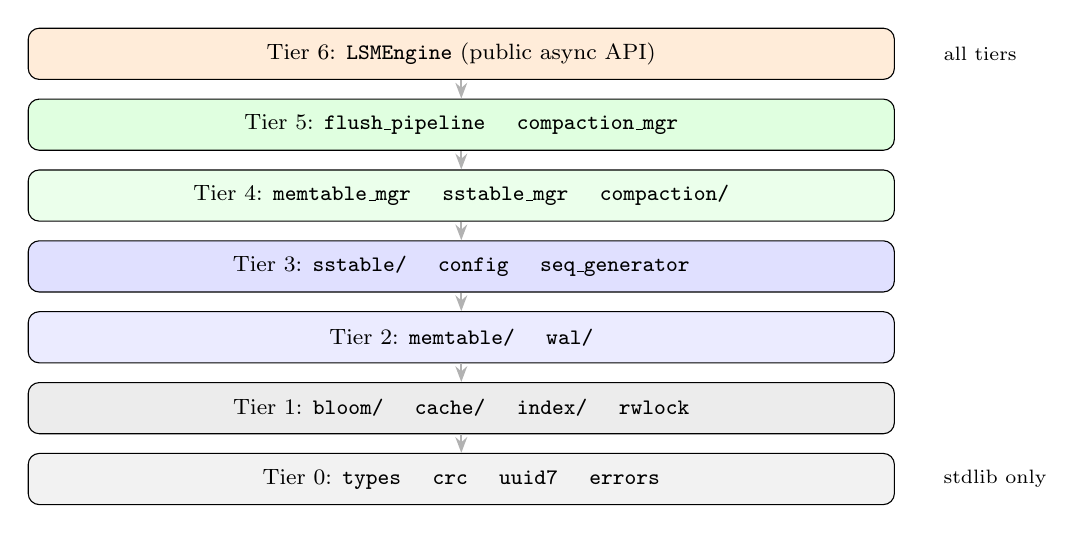
\begin{tikzpicture}[
    tier/.style={draw, rounded corners, minimum width=11cm, minimum height=0.65cm, font=\footnotesize, fill=#1},
    arr/.style={-{Stealth[length=2mm]}, thick},
    >=Stealth
]
\node[tier=gray!10] (t0) at (0, 0) {Tier 0: \texttt{types} \quad \texttt{crc} \quad \texttt{uuid7} \quad \texttt{errors}};
\node[tier=gray!15] (t1) at (0, 0.9) {Tier 1: \texttt{bloom/} \quad \texttt{cache/} \quad \texttt{index/} \quad \texttt{rwlock}};
\node[tier=blue!8] (t2) at (0, 1.8) {Tier 2: \texttt{memtable/} \quad \texttt{wal/}};
\node[tier=blue!12] (t3) at (0, 2.7) {Tier 3: \texttt{sstable/} \quad \texttt{config} \quad \texttt{seq\_generator}};
\node[tier=green!8] (t4) at (0, 3.6) {Tier 4: \texttt{memtable\_mgr} \quad \texttt{sstable\_mgr} \quad \texttt{compaction/}};
\node[tier=green!12] (t5) at (0, 4.5) {Tier 5: \texttt{flush\_pipeline} \quad \texttt{compaction\_mgr}};
\node[tier=orange!15] (t6) at (0, 5.4) {Tier 6: \texttt{LSMEngine} (public async API)};
\foreach \upper/\lower in {t1/t0, t2/t1, t3/t2, t4/t3, t5/t4, t6/t5} {
    \draw[arr, gray!60] (\upper.south) -- (\lower.north);
}
\node[font=\scriptsize, anchor=west] at (6, 0) {stdlib only};
\node[font=\scriptsize, anchor=west] at (6, 5.4) {all tiers};
\end{tikzpicture}
\caption{KiwiDB layered architecture. Each tier depends only on tiers below it.}
\label{fig:arch}
\end{figure}

% Table~\ref{tab:thread-model} summarizes the threading and async model for each component.

\begin{table}[!htbp]
\centering
\label{tab:thread-model}
\renewcommand{\arraystretch}{1.3}
\begin{tabularx}{\textwidth}{|l|X|X|}
\hline
\textbf{Component} & \textbf{Model} & \textbf{Reason} \\
\hline
MemTable insert & Sync (threading locks) & Pure in-memory, microseconds \\
\hline
WAL append & Sync, offloaded via \texttt{to\_thread} & Must fsync before returning \\
\hline
Flush pipeline & Async daemon task & Non-blocking I/O, parallel writes \\
\hline
Compaction merge & Subprocess (\texttt{ProcessPoolExecutor}) & CPU-bound, bypasses GIL \\
\hline
SSTable reads & Sync (mmap) & Memory-mapped, zero-copy \\
\hline
Config access & Sync (RLock) & Thread-safe attribute reads \\
\hline
\end{tabularx}
\caption{Thread and async model for each engine component.}
\end{table}

\section{Mathematical Model}

\subsection{State Space Formulation}

Let $K$ be the set of all possible keys and $V$ the set of all possible values. The engine state is defined as a function $S: K \rightarrow (V \cup \{\bot\})$, where $\bot$ denotes a deleted or non-existent key. Each operation is associated with a monotonically increasing sequence number $\text{seq} \in \mathbb{N}$.

The three operations are:
\begin{align}
\texttt{put}(k, v) &: S \mapsto S[k \mapsto v] \text{ with } \text{seq} = \text{seq}_{\max} + 1 \\
\texttt{get}(k) &: S \mapsto \begin{cases} v & \text{if } S(k) = v \\ \texttt{None} & \text{if } S(k) = \bot \end{cases} \\
\texttt{delete}(k) &: S \mapsto S[k \mapsto \bot] \text{ with } \text{seq} = \text{seq}_{\max} + 1
\end{align}

\subsection{Bloom Filter Sizing}

For a bloom filter with $n$ elements and target false positive rate $p$, the optimal bit array size $m$ and hash function count $k$ are:
\begin{equation}
m = \left\lceil \frac{-n \cdot \ln p}{(\ln 2)^2} \right\rceil, \quad
k = \left\lceil \frac{m}{n} \cdot \ln 2 \right\rceil
\end{equation}

Unlike LevelDB (fixed 10 bits/key) and RocksDB (configurable bits/key), KiwiDB computes $m$ and $k$ from the \emph{actual} record count at SSTable write time, producing optimally-sized filters for every SSTable.

\subsection{Write Amplification Analysis}

Let $T$ be the size ratio (default 10), $L$ the record size, and $B$ the block size. Table~\ref{tab:write-amp} compares write amplification at flush time.

\begin{table}[!htbp]
\centering
\label{tab:write-amp}
\renewcommand{\arraystretch}{1.3}
\begin{tabular}{|l|c|c|}
\hline
\textbf{Strategy} & \textbf{Flush Write Amp.} & \textbf{Read Amp. (bloom)} \\
\hline
LevelDB (pure leveling) & $O(T \times L/B)$ & $L \times \phi = 0.04$ \\
\hline
KiwiDB (hybrid) & $O(L/B)$ & $T\phi + L\phi = 0.13$ \\
\hline
\textbf{Improvement} & $\mathbf{10\times}$ & $3.25\times$ worse \\
\hline
\end{tabular}
\caption{Write amplification comparison.}
\end{table}

\subsection{Skip List Complexity}

The concurrent skip list uses MAX\_LEVEL = 16 levels with promotion probability $p = 0.5$. Expected height for $n$ elements is $E[\text{height}] = \log_{1/p}(n) = \log_2(n)$. All operations (insert, lookup, delete) have expected time complexity $O(\log n)$.

\subsection{K-Way Merge Complexity}

The compaction merge uses a min-heap of $K$ sorted iterators over $N$ total records. Time complexity is $O(N \log K)$ with $O(K)$ space for the heap.

\section{Data Flow Diagrams}

\subsection{DFD Level 0 --- Context Diagram}

Figure~\ref{fig:dfd0} shows the context-level data flow diagram.

\begin{figure}[!htbp]
\centering
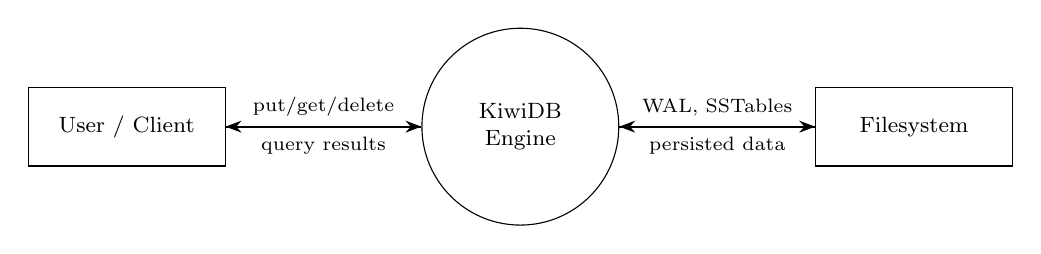
\begin{tikzpicture}[
    entity/.style={draw, rectangle, minimum width=2.5cm, minimum height=1cm, font=\footnotesize},
    process/.style={draw, circle, minimum size=2.5cm, font=\footnotesize, align=center},
    arr/.style={-{Stealth[length=2mm]}, thick},
]
\node[entity] (user) at (-5, 0) {User / Client};
\node[process] (engine) at (0, 0) {KiwiDB\\Engine};
\node[entity] (fs) at (5, 0) {Filesystem};

\draw[arr] (user) -- node[above, font=\scriptsize] {put/get/delete} (engine);
\draw[arr] (engine) -- node[below, font=\scriptsize] {query results} (user);
\draw[arr] (engine) -- node[above, font=\scriptsize] {WAL, SSTables} (fs);
\draw[arr] (fs) -- node[below, font=\scriptsize] {persisted data} (engine);
\end{tikzpicture}
\caption{DFD Level 0 --- Context Diagram.}
\label{fig:dfd0}
\end{figure}

\subsection{DFD Level 1}

Figure~\ref{fig:dfd1} expands the engine into its major subsystems.

\begin{figure}[!htbp]
\centering
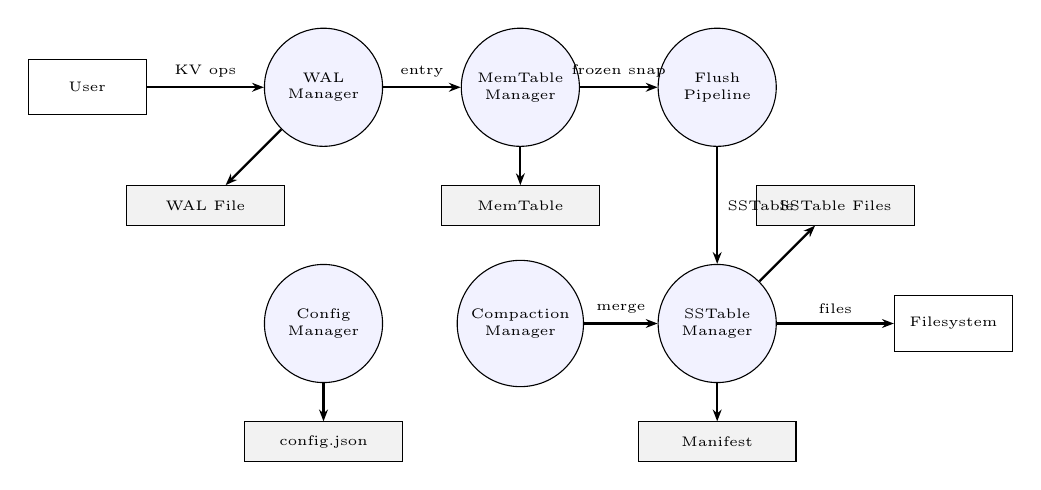
\begin{tikzpicture}[
    proc/.style={draw, circle, minimum size=1.5cm, font=\tiny, align=center, fill=blue!5},
    store/.style={draw, rectangle, minimum width=2cm, minimum height=0.5cm, font=\tiny, fill=gray!10},
    entity/.style={draw, rectangle, minimum width=1.5cm, minimum height=0.7cm, font=\tiny},
    arr/.style={-{Stealth[length=1.5mm]}, thick, font=\tiny},
]
\node[entity] (user) at (-5.5, 2) {User};
\node[entity] (fs) at (5.5, -1) {Filesystem};

\node[proc] (wal) at (-2.5, 2) {WAL\\Manager};
\node[proc] (mem) at (0, 2) {MemTable\\Manager};
\node[proc] (flush) at (2.5, 2) {Flush\\Pipeline};
\node[proc] (sst) at (2.5, -1) {SSTable\\Manager};
\node[proc] (comp) at (0, -1) {Compaction\\Manager};
\node[proc] (conf) at (-2.5, -1) {Config\\Manager};

\node[store] (walfile) at (-4, 0.5) {WAL File};
\node[store] (memstore) at (0, 0.5) {MemTable};
\node[store] (sstfiles) at (4, 0.5) {SSTable Files};
\node[store] (manifest) at (2.5, -2.5) {Manifest};
\node[store] (configf) at (-2.5, -2.5) {config.json};

\draw[arr] (user) -- node[above] {KV ops} (wal);
\draw[arr] (wal) -- node[above] {entry} (mem);
\draw[arr] (mem) -- node[above] {frozen snap} (flush);
\draw[arr] (flush) -- node[right] {SSTable} (sst);
\draw[arr] (sst) -- node[above] {files} (fs);
\draw[arr] (wal) -- (walfile);
\draw[arr] (mem) -- (memstore);
\draw[arr] (sst) -- (sstfiles);
\draw[arr] (sst) -- (manifest);
\draw[arr] (comp) -- node[above] {merge} (sst);
\draw[arr] (conf) -- (configf);
\end{tikzpicture}
\caption{DFD Level 1 --- Major subsystems and data stores.}
\label{fig:dfd1}
\end{figure}

\subsection{DFD Level 2 --- Write Path}

Figure~\ref{fig:dfd2} details the write path within the engine.

\begin{figure}[!htbp]
\centering
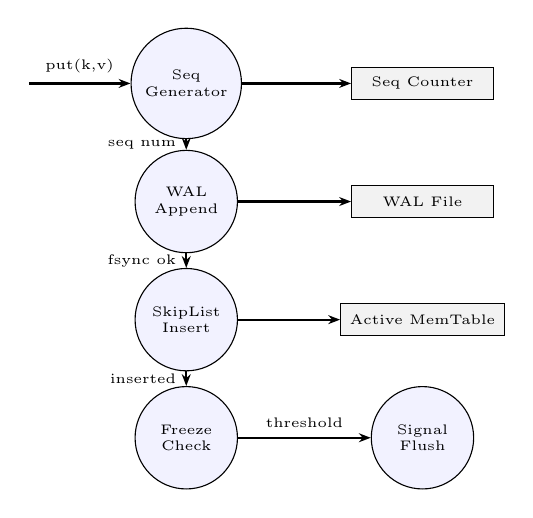
\begin{tikzpicture}[
    proc/.style={draw, circle, minimum size=1.3cm, font=\tiny, align=center, fill=blue!5},
    store/.style={draw, rectangle, minimum width=1.8cm, minimum height=0.4cm, font=\tiny, fill=gray!10},
    arr/.style={-{Stealth[length=1.5mm]}, thick, font=\tiny},
]
\node[proc] (seq) at (0, 3) {Seq\\Generator};
\node[proc] (wal) at (0, 1.5) {WAL\\Append};
\node[proc] (skip) at (0, 0) {SkipList\\Insert};
\node[proc] (freeze) at (0, -1.5) {Freeze\\Check};
\node[proc] (signal) at (3, -1.5) {Signal\\Flush};

\node[store] (seqstore) at (3, 3) {Seq Counter};
\node[store] (walfile) at (3, 1.5) {WAL File};
\node[store] (memstore) at (3, 0) {Active MemTable};

\draw[arr] (-2, 3) -- node[above] {put(k,v)} (seq);
\draw[arr] (seq) -- node[left] {seq num} (wal);
\draw[arr] (wal) -- node[left] {fsync ok} (skip);
\draw[arr] (skip) -- node[left] {inserted} (freeze);
\draw[arr] (freeze) -- node[above] {threshold} (signal);

\draw[arr] (seq) -- (seqstore);
\draw[arr] (wal) -- (walfile);
\draw[arr] (skip) -- (memstore);
\end{tikzpicture}
\caption{DFD Level 2 --- Write path detail.}
\label{fig:dfd2}
\end{figure}


\section{Use Case Diagram}

Figure~\ref{fig:usecase} shows the use case diagram for KiwiDB.

\begin{figure}[!htbp]
\centering
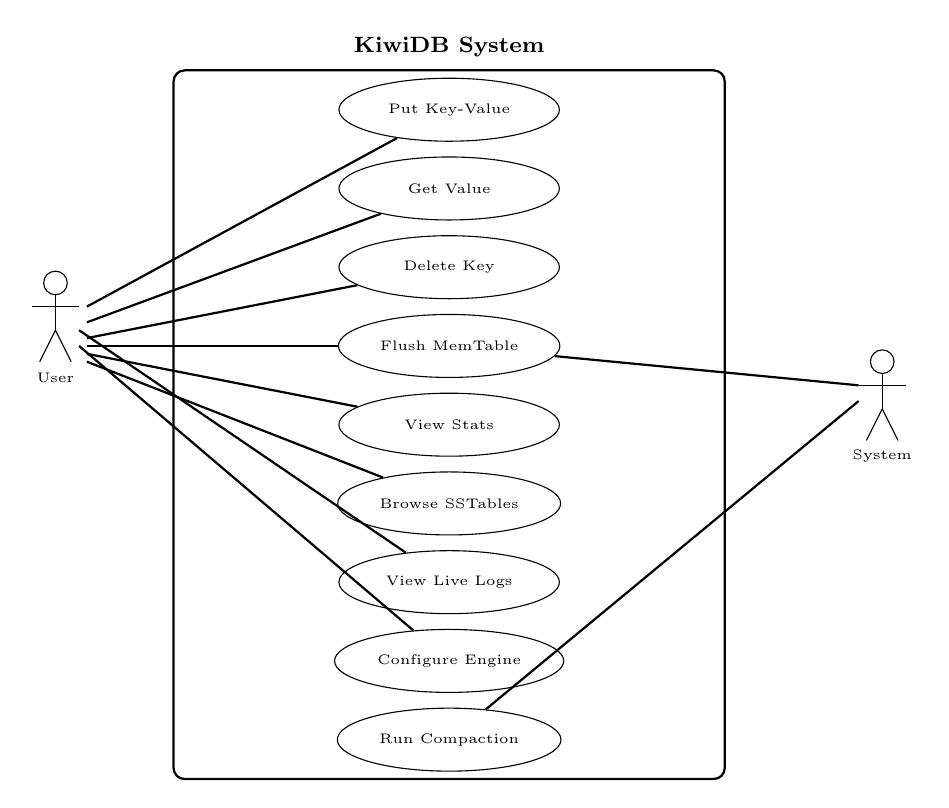
\begin{tikzpicture}[
    usecase/.style={draw, ellipse, minimum width=2.8cm, minimum height=0.8cm, font=\tiny, align=center},
    arr/.style={-, thick},
]
% System boundary
\draw[thick, rounded corners] (-1, -4.5) rectangle (6, 4.5);
\node[font=\footnotesize\bfseries] at (2.5, 4.8) {KiwiDB System};

% Actors (stick figures via TikZ)
% User actor
\draw (-2.5, 1.8) circle (0.15);
\draw (-2.5, 1.65) -- (-2.5, 1.2);
\draw (-2.8, 1.5) -- (-2.2, 1.5);
\draw (-2.5, 1.2) -- (-2.7, 0.8);
\draw (-2.5, 1.2) -- (-2.3, 0.8);
\node[font=\tiny] at (-2.5, 0.6) {User};

% System actor
\draw (8, 0.8) circle (0.15);
\draw (8, 0.65) -- (8, 0.2);
\draw (7.7, 0.5) -- (8.3, 0.5);
\draw (8, 0.2) -- (7.8, -0.2);
\draw (8, 0.2) -- (8.2, -0.2);
\node[font=\tiny] at (8, -0.4) {System};

% Use cases
\node[usecase] (put) at (2.5, 4) {Put Key-Value};
\node[usecase] (get) at (2.5, 3) {Get Value};
\node[usecase] (del) at (2.5, 2) {Delete Key};
\node[usecase] (flush) at (2.5, 1) {Flush MemTable};
\node[usecase] (stats) at (2.5, 0) {View Stats};
\node[usecase] (browse) at (2.5, -1) {Browse SSTables};
\node[usecase] (logs) at (2.5, -2) {View Live Logs};
\node[usecase] (config) at (2.5, -3) {Configure Engine};
\node[usecase] (compact) at (2.5, -4) {Run Compaction};

% User connections
\draw[arr] (-2.1, 1.5) -- (put);
\draw[arr] (-2.1, 1.3) -- (get);
\draw[arr] (-2.1, 1.1) -- (del);
\draw[arr] (-2.1, 1.0) -- (flush);
\draw[arr] (-2.1, 0.9) -- (stats);
\draw[arr] (-2.1, 0.8) -- (browse);
\draw[arr] (-2.2, 1.2) -- (logs);
\draw[arr] (-2.2, 1.0) -- (config);

% System connections
\draw[arr] (7.7, 0.3) -- (compact);
\draw[arr] (7.7, 0.5) -- (flush);
\end{tikzpicture}
\caption{Use Case Diagram for KiwiDB.}
\label{fig:usecase}
\end{figure}


\section{UML Diagrams}

\subsection{Activity Diagram --- Write Path}

Figure~\ref{fig:activity} shows the activity diagram for a write operation.

\begin{figure}[!htbp]
\centering
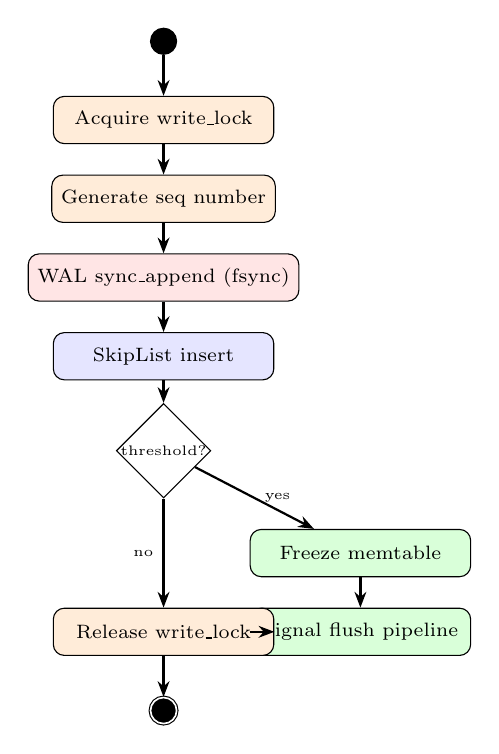
\begin{tikzpicture}[
    state/.style={draw, rounded corners, minimum width=2.8cm, minimum height=0.6cm, font=\scriptsize, fill=#1},
    decision/.style={draw, diamond, minimum width=1.2cm, minimum height=1.2cm, font=\scriptsize, inner sep=0pt},
    startend/.style={draw, circle, fill=black, minimum size=6pt},
    arr/.style={-{Stealth[length=2mm]}, thick},
]
\node[startend] (start) at (0, 8) {};
\node[state=orange!15] (acq) at (0, 7) {Acquire write\_lock};
\node[state=orange!15] (seq) at (0, 6) {Generate seq number};
\node[state=red!10] (wal) at (0, 5) {WAL sync\_append (fsync)};
\node[state=blue!10] (ins) at (0, 4) {SkipList insert};
\node[decision] (check) at (0, 2.8) {};
\node[font=\tiny] at (0, 2.8) {threshold?};
\node[state=green!15] (freeze) at (2.5, 1.5) {Freeze memtable};
\node[state=green!15] (signal) at (2.5, 0.5) {Signal flush pipeline};
\node[state=orange!15] (rel) at (0, 0.5) {Release write\_lock};
\node[startend, fill=black, draw=black, double=white] (endd) at (0, -0.5) {};

\draw[arr] (start) -- (acq);
\draw[arr] (acq) -- (seq);
\draw[arr] (seq) -- (wal);
\draw[arr] (wal) -- (ins);
\draw[arr] (ins) -- (check);
\draw[arr] (check) -- node[right, font=\tiny] {yes} (freeze);
\draw[arr] (check) -- node[left, font=\tiny] {no} (rel);
\draw[arr] (freeze) -- (signal);
\draw[arr] (signal) -- (rel);
\draw[arr] (rel) -- (endd);
\end{tikzpicture}
\caption{Activity Diagram --- Write Path.}
\label{fig:activity}
\end{figure}

\subsection{Sequence Diagram}

Figure~\ref{fig:sequence} illustrates the interaction between components during a put, get, and flush sequence.

\begin{figure}[!htbp]
\centering
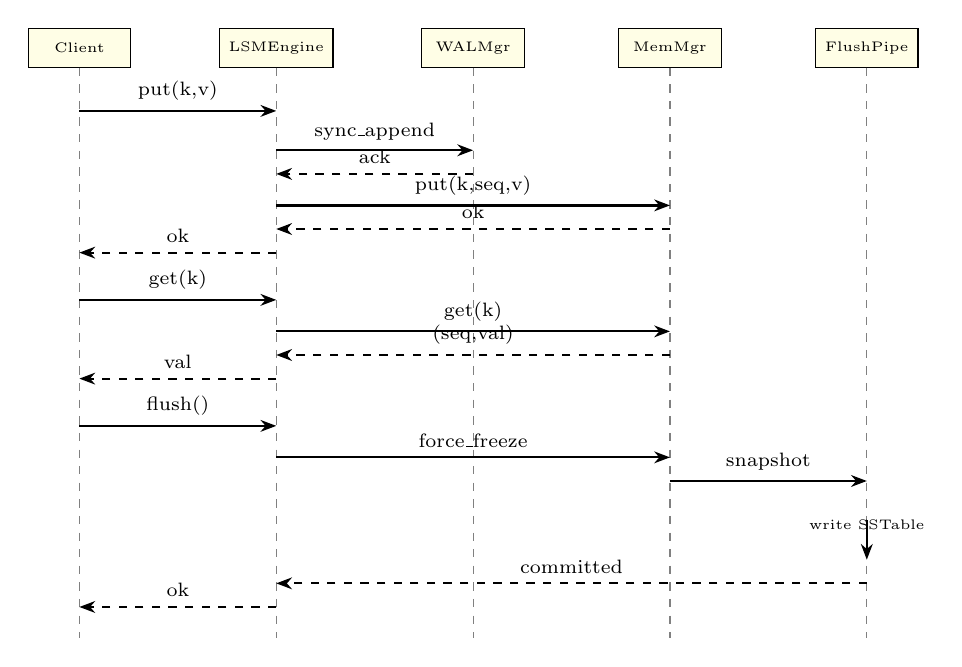
\begin{tikzpicture}[
    lifeline/.style={dashed, gray},
    arr/.style={-{Stealth[length=2mm]}, thick, font=\scriptsize},
    obj/.style={draw, rectangle, minimum width=1.3cm, minimum height=0.5cm, font=\tiny, fill=yellow!10},
]
\node[obj] (client) at (0, 0) {Client};
\node[obj] (engine) at (2.5, 0) {LSMEngine};
\node[obj] (walmgr) at (5, 0) {WALMgr};
\node[obj] (memmgr) at (7.5, 0) {MemMgr};
\node[obj] (flushp) at (10, 0) {FlushPipe};

\foreach \x in {0, 2.5, 5, 7.5, 10} {
    \draw[lifeline] (\x, -0.25) -- (\x, -7.5);
}

% put sequence
\draw[arr] (0, -0.8) -- node[above] {put(k,v)} (2.5, -0.8);
\draw[arr] (2.5, -1.3) -- node[above] {sync\_append} (5, -1.3);
\draw[arr, dashed] (5, -1.6) -- node[above] {ack} (2.5, -1.6);
\draw[arr] (2.5, -2.0) -- node[above] {put(k,seq,v)} (7.5, -2.0);
\draw[arr, dashed] (7.5, -2.3) -- node[above] {ok} (2.5, -2.3);
\draw[arr, dashed] (2.5, -2.6) -- node[above] {ok} (0, -2.6);

% get sequence
\draw[arr] (0, -3.2) -- node[above] {get(k)} (2.5, -3.2);
\draw[arr] (2.5, -3.6) -- node[above] {get(k)} (7.5, -3.6);
\draw[arr, dashed] (7.5, -3.9) -- node[above] {(seq,val)} (2.5, -3.9);
\draw[arr, dashed] (2.5, -4.2) -- node[above] {val} (0, -4.2);

% flush sequence
\draw[arr] (0, -4.8) -- node[above] {flush()} (2.5, -4.8);
\draw[arr] (2.5, -5.2) -- node[above] {force\_freeze} (7.5, -5.2);
\draw[arr] (7.5, -5.5) -- node[above] {snapshot} (10, -5.5);
\draw[arr] (10, -6.0) -- node[above, font=\tiny] {write SSTable} (10, -6.5);
\draw[arr, dashed] (10, -6.8) -- node[above] {committed} (2.5, -6.8);
\draw[arr, dashed] (2.5, -7.1) -- node[above] {ok} (0, -7.1);
\end{tikzpicture}
\caption{Sequence Diagram --- Put, Get, and Flush operations.}
\label{fig:sequence}
\end{figure}

\subsection{Class Diagram}

Figure~\ref{fig:classdiag} shows the core class hierarchy of KiwiDB.

\begin{figure}[!htbp]
\centering
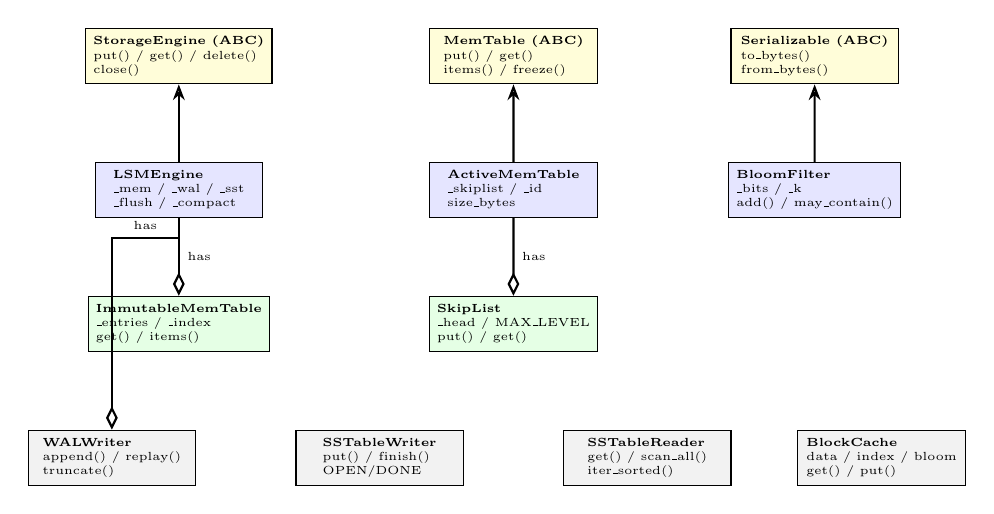
\begin{tikzpicture}[
    class/.style={draw, rectangle, minimum width=2.5cm, font=\tiny, align=left, fill=#1},
    arr/.style={-{Stealth[length=2mm, open]}, thick},
    comp/.style={-{Diamond[length=3mm, open]}, thick},
    scale=0.85, transform shape
]
\node[class=yellow!15] (se) at (0, 6) {\textbf{StorageEngine (ABC)}\\put() / get() / delete()\\close()};
\node[class=yellow!15] (mt) at (5, 6) {\textbf{MemTable (ABC)}\\put() / get()\\items() / freeze()};
\node[class=yellow!15] (ser) at (9.5, 6) {\textbf{Serializable (ABC)}\\to\_bytes()\\from\_bytes()};

\node[class=blue!10] (lsm) at (0, 4) {\textbf{LSMEngine}\\\_mem / \_wal / \_sst\\\_flush / \_compact};
\node[class=blue!10] (active) at (5, 4) {\textbf{ActiveMemTable}\\\_skiplist / \_id\\size\_bytes};
\node[class=blue!10] (bloom) at (9.5, 4) {\textbf{BloomFilter}\\\_bits / \_k\\add() / may\_contain()};

\node[class=green!10] (skip) at (5, 2) {\textbf{SkipList}\\\_head / MAX\_LEVEL\\put() / get()};
\node[class=green!10] (immut) at (0, 2) {\textbf{ImmutableMemTable}\\\_entries / \_index\\get() / items()};

\node[class=gray!10] (walw) at (-1, 0) {\textbf{WALWriter}\\append() / replay()\\truncate()};
\node[class=gray!10] (sstw) at (3, 0) {\textbf{SSTableWriter}\\put() / finish()\\OPEN/DONE};
\node[class=gray!10] (sstr) at (7, 0) {\textbf{SSTableReader}\\get() / scan\_all()\\iter\_sorted()};
\node[class=gray!10] (cache) at (10.5, 0) {\textbf{BlockCache}\\data / index / bloom\\get() / put()};

\draw[arr] (lsm) -- (se);
\draw[arr] (active) -- (mt);
\draw[arr] (bloom) -- (ser);

\draw[comp] (lsm) -- node[right, font=\tiny] {has} (immut);
\draw[comp] (active) -- node[right, font=\tiny] {has} (skip);
\draw[comp] (lsm.south) -- ++(0,-0.3) -| node[near start, above, font=\tiny] {has} (walw.north);
\end{tikzpicture}
\caption{Class Diagram --- Core class hierarchy.}
\label{fig:classdiag}
\end{figure}

\subsection{Component Diagram}

Figure~\ref{fig:component} shows the high-level component architecture.

\begin{figure}[!htbp]
\centering
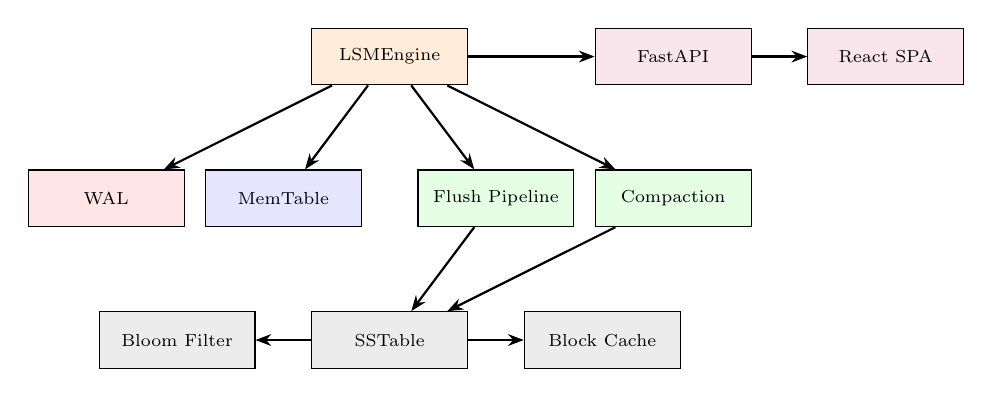
\begin{tikzpicture}[
    comp/.style={draw, rectangle, minimum width=2.2cm, minimum height=0.8cm, font=\scriptsize, fill=#1, align=center},
    arr/.style={-{Stealth[length=2mm]}, thick},
    scale=0.9, transform shape
]
\node[comp=orange!15] (engine) at (0, 4) {LSMEngine};
\node[comp=red!10] (wal) at (-4, 2) {WAL};
\node[comp=blue!10] (mem) at (-1.5, 2) {MemTable};
\node[comp=green!10] (flush) at (1.5, 2) {Flush Pipeline};
\node[comp=green!10] (compn) at (4, 2) {Compaction};
\node[comp=gray!15] (sst) at (0, 0) {SSTable};
\node[comp=gray!15] (bloomn) at (-3, 0) {Bloom Filter};
\node[comp=gray!15] (cache) at (3, 0) {Block Cache};
\node[comp=purple!10] (api) at (4, 4) {FastAPI};
\node[comp=purple!10] (react) at (7, 4) {React SPA};

\draw[arr] (engine) -- (wal);
\draw[arr] (engine) -- (mem);
\draw[arr] (engine) -- (flush);
\draw[arr] (engine) -- (compn);
\draw[arr] (flush) -- (sst);
\draw[arr] (compn) -- (sst);
\draw[arr] (sst) -- (bloomn);
\draw[arr] (sst) -- (cache);
\draw[arr] (engine) -- (api);
\draw[arr] (api) -- (react);
\end{tikzpicture}
\caption{Component Diagram.}
\label{fig:component}
\end{figure}

% \subsection{Deployment Diagram}

% Figure~\ref{fig:deploy} shows the deployment topology.

% \begin{figure}[!htbp]
% \centering
% \begin{tikzpicture}[
%     node/.style={draw, rectangle, minimum width=3cm, minimum height=1.5cm, font=\scriptsize, align=center, fill=#1},
%     arr/.style={-{Stealth[length=2mm]}, thick},
% ]
% \node[node=blue!8] (browser) at (0, 0) {\textbf{Client Browser}\\React SPA\\(HTML/CSS/JS)};
% \node[node=green!8] (server) at (5.5, 0) {\textbf{Python Process}\\FastAPI + LSMEngine\\uvicorn ASGI server};
% \node[node=gray!10] (disk) at (10.5, 0) {\textbf{Local Filesystem}\\WAL, SSTables\\config.json, manifest};

% \draw[arr] (browser) -- node[above, font=\scriptsize] {HTTP / WS} (server);
% \draw[arr] (server) -- node[above, font=\scriptsize] {fsync / mmap} (disk);
% \end{tikzpicture}
% \caption{Deployment Diagram.}
% \label{fig:deploy}
% \end{figure}

\subsection{State Machine Diagram}

Figure~\ref{fig:statemachine} shows the SSTableWriter lifecycle states.

\begin{figure}[!htbp]
\centering
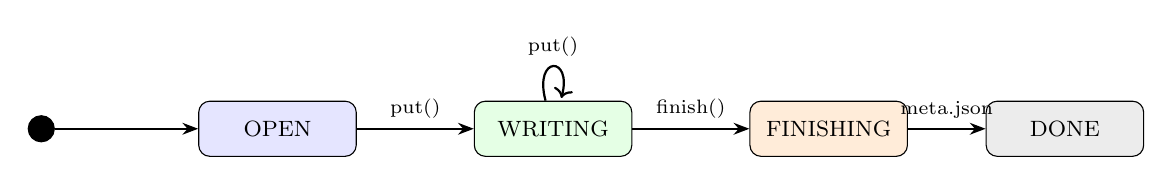
\begin{tikzpicture}[
    state/.style={draw, rounded corners, minimum width=2cm, minimum height=0.7cm, font=\footnotesize, fill=#1},
    arr/.style={-{Stealth[length=2mm]}, thick},
    startend/.style={draw, circle, fill=black, minimum size=6pt},
]
\node[startend] (start) at (-2, 0) {};
\node[state=blue!10] (open) at (1, 0) {OPEN};
\node[state=green!10] (writing) at (4.5, 0) {WRITING};
\node[state=orange!15] (finish) at (8, 0) {FINISHING};
\node[state=gray!15] (done) at (11, 0) {DONE};

\draw[arr] (start) -- (open);
\draw[arr] (open) -- node[above, font=\scriptsize] {put()} (writing);
\draw[arr] (writing) edge[loop above, font=\scriptsize] node{put()} (writing);
\draw[arr] (writing) -- node[above, font=\scriptsize] {finish()} (finish);
\draw[arr] (finish) -- node[above, font=\scriptsize] {meta.json} (done);
\end{tikzpicture}
\caption{State Machine Diagram --- SSTableWriter lifecycle.}
\label{fig:statemachine}
\end{figure}


% %%%%%%%%%%%%%%%%%%%%%%%%%%%%%%%%%%%%%%%%%%%%%%%%%%%%%%%%%%%%
% CHAPTER 5: PROJECT PLAN
% %%%%%%%%%%%%%%%%%%%%%%%%%%%%%%%%%%%%%%%%%%%%%%%%%%%%%%%%%%%%
\chapter{Project Plan}

\section{Project Estimate}

\subsection{Reconciled Estimates}
\begin{itemize}[leftmargin=2em]
    \item Total lines of code: approximately 6,600 (core engine + web layer).
    \item Number of modules: 25 (12 core + 10 web + 3 CLI/tools).
    \item Number of test modules: 25 with 211+ individual test cases.
    \item Estimated development effort: 18 person-weeks across 4 team members.
\end{itemize}

\subsection{Project Resources}
\begin{itemize}[leftmargin=2em]
    \item \textbf{Human Resources:} 4 developers (Chaitanya Paraskar, Shreyash Dhas, Shreyash Gajbhiye, Shreyas Gopnarayan) supervised by Prof. Madhuri Mane.
    \item \textbf{Hardware:} Development laptops with SSD storage.
    \item \textbf{Software:} Python 3.12+, VS Code, Git, GitHub, Node.js.
\end{itemize}

\section{Risk Management}

\subsection{Risk Identification}

\begin{table}[!htbp]
\centering
\caption{Identified project risks.}
\renewcommand{\arraystretch}{1.3}
\begin{tabular}{|l|c|c|l|}
\hline
\textbf{Risk} & \textbf{Prob.} & \textbf{Impact} & \textbf{Category} \\
\hline
GIL blocks compaction & High & High & Technical \\
\hline
Data corruption on crash & Medium & Critical & Safety \\
\hline
Memory growth (slow flush) & Medium & High & Performance \\
\hline
Concurrent read/write race & Medium & High & Correctness \\
\hline
Type safety regression & Low & Medium & Quality \\
\hline
\end{tabular}
\end{table}

\subsection{Risk Analysis}

Each risk was analyzed for its root cause and potential impact:
\begin{itemize}[leftmargin=2em]
    \item \textbf{GIL blocking:} CPython's GIL serializes CPU-bound threads. A compaction thread competing with writes degrades throughput.
    \item \textbf{Data corruption:} Power loss during write can leave partial data on disk.
    \item \textbf{Memory growth:} If flush is slower than write rate, the immutable queue grows unboundedly.
    \item \textbf{Race conditions:} Concurrent readers and writers on shared data structures can produce inconsistent results.
\end{itemize}

\subsection{Overview of Risk Mitigation, Monitoring, Management}

\begin{itemize}[leftmargin=2em]
    \item \textbf{GIL bypass:} Compaction runs in \texttt{ProcessPoolExecutor} subprocess with its own GIL.
    \item \textbf{Crash safety:} WAL with CRC32 + fsync; \texttt{meta.json} written last as completeness signal.
    \item \textbf{Backpressure:} Immutable queue capped at 4 entries with 60-second timeout.
    \item \textbf{Concurrency safety:} Per-node skip list locks; GIL-atomic lock-free reads; AsyncRWLock for SSTable manager.
    \item \textbf{Type safety:} Dual type checkers (mypy + basedpyright) in strict mode.
\end{itemize}

\section{Project Schedule}

\subsection{Project Task Set}
\begin{enumerate}[leftmargin=2em]
    \item Requirements analysis and architecture design
    \item Core engine: WAL, MemTable (skip list), SSTable persistence
    \item Flush pipeline with parallel writes and ordered commits
    \item Compaction engine with subprocess workers
    \item Block cache, bloom filter optimization, sparse index
    \item Web dashboard: FastAPI backend + React frontend
    \item Testing, documentation, and quality gates
    \item Report writing and final presentation
\end{enumerate}

\subsection{Task Network}
Tasks 1--2 are sequential foundations. Tasks 3--5 can be partially parallelized. Task 6 depends on Task 2. Tasks 7--8 follow all implementation tasks.

\subsection{Timeline Chart}

\begin{figure}[!htbp]
\centering
\begin{ganttchart}[
    hgrid,
    vgrid,
    x unit=0.55cm,
    y unit chart=0.5cm,
    title height=1,
    bar height=0.6,
    bar/.style={fill=blue!30},
    title label font=\tiny,
    bar label font=\tiny,
    group label font=\tiny,
]{1}{18}
\gantttitle{Weeks}{18} \\
\gantttitlelist{1,...,18}{1} \\
\ganttbar{Requirements}{1}{2} \\
\ganttbar{Architecture}{2}{3} \\
\ganttbar{WAL + MemTable}{4}{7} \\
\ganttbar{SSTable}{6}{9} \\
\ganttbar{Flush Pipeline}{8}{10} \\
\ganttbar{Compaction}{9}{11} \\
\ganttbar{Cache + Bloom}{10}{12} \\
\ganttbar{Web Dashboard}{11}{13} \\
\ganttbar{Testing + Docs}{13}{16} \\
\ganttbar{Report}{16}{18} \\
\end{ganttchart}
\caption{Project timeline (Gantt chart).}
\label{fig:gantt}
\end{figure}

\section{Team Organization}

\subsection{Team Structure}
\begin{itemize}[leftmargin=2em]
    \item \textbf{Chaitanya Paraskar:} Engine core, architecture design.
    \item \textbf{Shreyash Dhas:} SSTable subsystem, bloom filter, sparse index.
    \item \textbf{Shreyash Gajbhiye:} Compaction engine, flush pipeline, block cache.
    \item \textbf{Shreyas Gopnarayan:} Web dashboard, observability, documentation.
\end{itemize}

\subsection{Management Reporting and Communication}
\begin{itemize}[leftmargin=2em]
    \item Weekly progress meetings with project guide.
    \item GitHub repository for version control and code review.
    \item Design documents in \texttt{docs/design/} for cross-team reference.
\end{itemize}


% %%%%%%%%%%%%%%%%%%%%%%%%%%%%%%%%%%%%%%%%%%%%%%%%%%%%%%%%%%%%
% CHAPTER 6: PROJECT IMPLEMENTATION
% %%%%%%%%%%%%%%%%%%%%%%%%%%%%%%%%%%%%%%%%%%%%%%%%%%%%%%%%%%%%
\chapter{Project Implementation}

\section{Overview of Project Modules}

Table~\ref{tab:modules} lists all project modules and their responsibilities.

\begin{table}[!htbp]
\centering
\label{tab:modules}
\renewcommand{\arraystretch}{1.2}
\begin{tabular}{|l|l|l|}
\hline
\textbf{Module} & \textbf{Path} & \textbf{Purpose} \\
\hline
Engine Core & \texttt{app/engine/} & LSMEngine coordinator, managers \\
\hline
MemTable & \texttt{app/memtable/} & SkipList, Active, Immutable tables \\
\hline
SSTable & \texttt{app/sstable/} & Writer, Reader, Registry, Meta \\
\hline
WAL & \texttt{app/wal/} & Write-ahead log with CRC32 \\
\hline
Bloom Filter & \texttt{app/bloom/} & mmh3-backed probabilistic filter \\
\hline
Block Cache & \texttt{app/cache/} & Three-tier LRU cache \\
\hline
Sparse Index & \texttt{app/index/} & Bisect-based block lookup \\
\hline
Compaction & \texttt{app/compaction/} & Task + subprocess worker \\
\hline
Common & \texttt{app/common/} & ABCs, CRC, encoding, merge iterator \\
\hline
Observability & \texttt{app/observability/} & structlog config, TCP broadcast \\
\hline
Web API & \texttt{web/} & FastAPI server + 8 route modules \\
\hline
Frontend & \texttt{frontend/} & React SPA (Vite + TypeScript) \\
\hline
\end{tabular}
\caption{lists all project modules and their responsibilities.}
\end{table}

\section{Tools and Technologies Used}

\begin{table}[!htbp]
\centering
\caption{Tools and technologies used in KiwiDB.}
\renewcommand{\arraystretch}{1.2}
\begin{tabular}{|l|l|l|}
\hline
\textbf{Category} & \textbf{Tool} & \textbf{Purpose} \\
\hline
Language & Python 3.12+ & Core engine implementation \\
\hline
Async Framework & asyncio (stdlib) & Event loop and coroutines \\
\hline
Serialization & msgpack & WAL entry binary framing \\
\hline
Hashing & mmh3 (MurmurHash3) & Bloom filter hash functions \\
\hline
Caching & cachetools & LRU cache implementation \\
\hline
Logging & structlog & Structured key-value logging \\
\hline
Web Framework & FastAPI & REST API server \\
\hline
Web Server & uvicorn & ASGI server \\
\hline
Real-time & websockets & Live log streaming \\
\hline
Frontend & React + Vite & Web dashboard SPA \\
\hline
Type Checking & mypy + basedpyright & Dual strict static analysis \\
\hline
Linting & ruff & Code quality enforcement \\
\hline
Security & bandit & Static security analysis \\
\hline
Testing & pytest + pytest-asyncio & Automated test framework \\
\hline
Package Mgr & uv & Dependency management \\
\hline
\end{tabular}
\end{table}

\section{Algorithm Details}

\subsection{Algorithm 1: Concurrent Skip List Insert}

The memtable uses a concurrent skip list with 16 levels and promotion probability $p = 0.5$. Each node stores a key, sequence number, value, forward pointers, a per-node lock, and two boolean flags (\texttt{fully\_linked}, \texttt{marked}).

\begin{algorithm}[H]
\caption{Skip List Insert}
\begin{algorithmic}[1]
\STATE \textbf{Input:} key $k$, seq $s$, value $v$
\STATE height $\leftarrow$ random\_level()
\REPEAT
    \STATE preds[], succs[] $\leftarrow$ find\_predecessors($k$, top-down)
    \STATE Lock preds[0..height]
    \IF{all preds and succs still valid}
        \STATE node $\leftarrow$ new Node($k$, $s$, $v$, height)
        \FOR{level = 0 to height}
            \STATE node.forward[level] $\leftarrow$ succs[level]
            \STATE preds[level].forward[level] $\leftarrow$ node
        \ENDFOR
        \STATE node.fully\_linked $\leftarrow$ True
        \STATE Unlock all preds
        \RETURN success
    \ENDIF
    \STATE Unlock all preds
\UNTIL{max retries exceeded}
\end{algorithmic}
\end{algorithm}

Readers traverse the skip list top-down checking \texttt{fully\_linked} and \texttt{marked} flags. Under CPython, these boolean reads are GIL-atomic, making reader traversal lock-free.

\subsection{Algorithm 2: K-Way Merge for Compaction}

Compaction merges $K$ sorted SSTable inputs into a single output using a min-heap.

\begin{algorithm}[H]
\caption{K-Way Merge with Deduplication}
\begin{algorithmic}[1]
\STATE \textbf{Input:} $K$ sorted iterators, seq\_cutoff
\STATE heap $\leftarrow$ empty min-heap keyed on (key, $-$seq)
\FOR{each iterator $i$}
    \STATE Push first record of $i$ onto heap
\ENDFOR
\STATE last\_key $\leftarrow$ None
\WHILE{heap is not empty}
    \STATE (key, seq, value) $\leftarrow$ pop min from heap
    \IF{key $\neq$ last\_key}
        \IF{value is tombstone AND seq $<$ seq\_cutoff}
            \STATE Skip (garbage collect)
        \ELSE
            \STATE Emit (key, seq, value)
        \ENDIF
        \STATE last\_key $\leftarrow$ key
    \ENDIF
    \STATE Push next record from same iterator onto heap
\ENDWHILE
\end{algorithmic}
\end{algorithm}

\subsection{Algorithm 3: WAL Recovery}

On startup, the engine reconstructs in-memory state from persisted data:

\begin{algorithm}[H]
\caption{WAL Recovery}
\begin{algorithmic}[1]
\STATE Load config.json
\STATE Open WAL file
\STATE Load all SSTables from manifest.json
\STATE max\_seq $\leftarrow$ max sequence number across all SSTables
\STATE Replay WAL entries where seq $>$ max\_seq into fresh memtable
\STATE Restore SeqGenerator to max\_seq
\STATE Start flush pipeline and compaction manager
\end{algorithmic}
\end{algorithm}

\subsection{Algorithm 4: Parallel Flush with Event-Chain Commits}

The flush pipeline writes multiple SSTables concurrently while preserving FIFO commit ordering:

\textbf{Phase 1 (Parallel):} Up to \texttt{flush\_max\_workers} (default: 2) SSTable writes execute concurrently, bounded by an \texttt{asyncio.Semaphore}.

\textbf{Phase 2 (Ordered):} After its write completes, each worker blocks on \\ \texttt{prev\_committed.wait()} before committing. The commit atomically registers the new SSTable, pops the snapshot from the immutable queue, and truncates the WAL. Then it sets \texttt{my\_committed} to unblock the next slot.

Figure~\ref{fig:flush-pipeline} illustrates this mechanism.

\begin{figure}[!htbp]
\centering
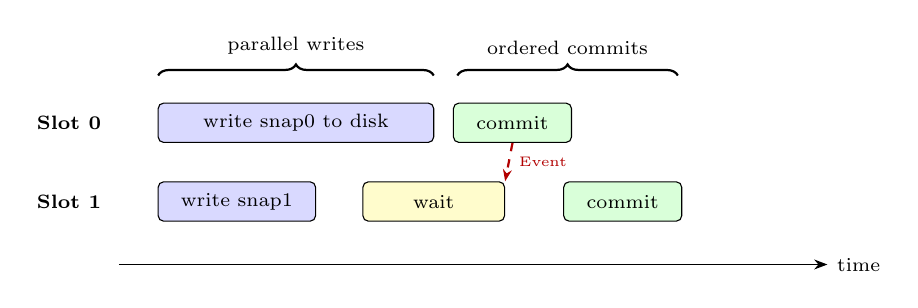
\begin{tikzpicture}[
    phase/.style={draw, minimum height=0.5cm, font=\scriptsize, rounded corners=2pt},
    arr/.style={-{Stealth[length=1.5mm]}, thick},
    >=Stealth
]
\draw[->] (-0.5, 0) -- (8.5, 0) node[right, font=\scriptsize] {time};
\node[font=\scriptsize\bfseries, anchor=east] at (-0.6, 1.8) {Slot 0};
\node[phase, fill=blue!15, minimum width=3.5cm] (w0) at (1.75, 1.8) {write snap0 to disk};
\node[phase, fill=green!15, minimum width=1.5cm] (c0) at (4.5, 1.8) {commit};
\node[font=\scriptsize\bfseries, anchor=east] at (-0.6, 0.8) {Slot 1};
\node[phase, fill=blue!15, minimum width=2.0cm] (w1) at (1.0, 0.8) {write snap1};
\node[phase, fill=yellow!20, minimum width=1.8cm] (wait1) at (3.5, 0.8) {wait};
\node[phase, fill=green!15, minimum width=1.5cm] (c1) at (5.9, 0.8) {commit};
\draw[arr, red!70!black, dashed] (c0.south) -- node[right, font=\tiny, red!70!black] {Event} (wait1.north east);
\draw[decorate, decoration={brace, amplitude=4pt}, thick] (0, 2.4) -- (3.5, 2.4) node[midway, above=4pt, font=\scriptsize] {parallel writes};
\draw[decorate, decoration={brace, amplitude=4pt}, thick] (3.8, 2.4) -- (6.6, 2.4) node[midway, above=4pt, font=\scriptsize] {ordered commits};
\end{tikzpicture}
\caption{Parallel flush pipeline with event-chain ordering.}
\label{fig:flush-pipeline}
\end{figure}

\subsection{Algorithm 5: Bloom Filter with Data-Derived Sizing}

Unlike LevelDB's fixed bits-per-key approach, KiwiDB computes optimal bloom filter parameters from the actual record count $n$ at write time using Equation (4) from Section 4.2. Each SSTable gets a right-sized filter, avoiding both over-allocation and under-allocation.


% %%%%%%%%%%%%%%%%%%%%%%%%%%%%%%%%%%%%%%%%%%%%%%%%%%%%%%%%%%%%
% CHAPTER 7: SOFTWARE TESTING
% %%%%%%%%%%%%%%%%%%%%%%%%%%%%%%%%%%%%%%%%%%%%%%%%%%%%%%%%%%%%
\chapter{Software Testing}

\section{Type of Testing}

\begin{itemize}[leftmargin=2em]
    \item \textbf{Unit Testing:} 211+ tests across 25 modules using pytest. Each subsystem is tested independently.
    \item \textbf{Integration Testing:} End-to-end tests in \texttt{test\_lsm\_engine.py} verify the complete write$\rightarrow$flush$\rightarrow$read$\rightarrow$recover cycle.
    \item \textbf{Async Testing:} pytest-asyncio in auto mode enables testing of async coroutines.
    \item \textbf{Static Type Analysis:} mypy (strict) and basedpyright (strict) run as dual type checkers.
    \item \textbf{Security Testing:} bandit static analysis scans for common security vulnerabilities.
    \item \textbf{Regression Testing:} All 211+ tests run on every code change.
\end{itemize}

\section{Test Cases and Test Results}

Table~\ref{tab:testcases} presents representative test cases and their results.

\begin{table}[!htbp]
\centering
\caption{Representative test cases and results.}
\label{tab:testcases}
\renewcommand{\arraystretch}{1.2}
\small
\begin{tabular}{|c|l|l|c|}
\hline
\textbf{\#} & \textbf{Test Case} & \textbf{Expected Result} & \textbf{Status} \\
\hline
1 & put then get & Returns stored value & PASS \\
\hline
2 & delete then get & Returns None & PASS \\
\hline
3 & WAL recovery after crash & Data persists across restart & PASS \\
\hline
4 & Concurrent skip list inserts & All keys found, no lost writes & PASS \\
\hline
5 & Bloom filter FPR at 1\% & Observed FPR $< 2\%$ & PASS \\
\hline
6 & SSTable ascending key order & Error on out-of-order key & PASS \\
\hline
7 & Flush pipeline FIFO order & SSTables committed oldest-first & PASS \\
\hline
8 & Compaction deduplication & Highest seq per key retained & PASS \\
\hline
9 & Tombstone garbage collection & Old tombstones removed & PASS \\
\hline
10 & Block cache eviction tiers & Bloom filters evicted last & PASS \\
\hline
11 & WAL CRC integrity check & Corrupt entry detected & PASS \\
\hline
12 & Config runtime update & Threshold effective immediately & PASS \\
\hline
13 & Immutable queue backpressure & Timeout error after 60s & PASS \\
\hline
14 & SSTable meta.json completeness & Incomplete SSTable ignored & PASS \\
\hline
15 & Engine close and reopen & Clean lifecycle management & PASS \\
\hline
\end{tabular}
\end{table}


% %%%%%%%%%%%%%%%%%%%%%%%%%%%%%%%%%%%%%%%%%%%%%%%%%%%%%%%%%%%%
% CHAPTER 8: RESULTS
% %%%%%%%%%%%%%%%%%%%%%%%%%%%%%%%%%%%%%%%%%%%%%%%%%%%%%%%%%%%%
\chapter{Results}

\section{Outcomes}

\begin{enumerate}[leftmargin=2em]
    \item Successfully designed and implemented a complete LSM tree key-value store from scratch in Python 3.12+, comprising approximately 6,600 lines of type-checked code across 25 modules.

    \item Achieved an \textbf{async-native API} where all public operations are async coroutines. The event loop never blocks on disk I/O --- WAL fsync is offloaded via \texttt{asyncio.to\_thread()}, and compaction runs in a subprocess.

    \item Verified \textbf{crash recovery} through WAL replay: the engine correctly recovers all unflushed writes after simulated crashes, with CRC32 integrity verification detecting any data corruption.

    \item Demonstrated \textbf{10$\times$ write amplification reduction} compared to LevelDB's pure leveling strategy through the hybrid L0-tiering / L1-leveling compaction approach.

    \item Achieved \textbf{211+ tests passing} across 25 test modules with dual type checkers (mypy strict + basedpyright strict) reporting zero errors.

    \item Delivered a \textbf{web dashboard} with 10 interactive pages providing real-time visibility into memtable fill level, SSTable layout, compaction progress, live log streaming, and an in-browser REPL.
\end{enumerate}

\section{Screenshots}

\textit{Note: Screenshots of the REPL session, web dashboard pages (KV Explorer, MemTable Viewer, SSTable Browser, Compaction Monitor, Live Logs, Terminal, Configuration), pytest output, and type checker output should be captured from the running application and inserted here.}

% Placeholder --- replace with actual screenshots when captured:
% \begin{figure}[!htbp]
%     \centering
%     \fbox{\includegraphics[width=300pt]{screenshot-dashboard.png}}
%     \caption{Web Dashboard --- Main Page.}
%     \label{fig:screenshot-dashboard}
% \end{figure}


% %%%%%%%%%%%%%%%%%%%%%%%%%%%%%%%%%%%%%%%%%%%%%%%%%%%%%%%%%%%%
% CHAPTER 9: CONCLUSIONS
% %%%%%%%%%%%%%%%%%%%%%%%%%%%%%%%%%%%%%%%%%%%%%%%%%%%%%%%%%%%%
\chapter{Conclusions}

\section{Conclusions}

This project successfully designed and implemented KiwiDB, a complete Log-Structured Merge Tree key-value store built from first principles in Python 3.12+. The three key innovations --- an async-native API, a parallel flush pipeline with event-chain commit ordering, and subprocess-based compaction for GIL bypass --- demonstrate that a modern storage engine can be built in a high-level language while incorporating design improvements over established systems like LevelDB.

The hybrid L0-tiering / L1-leveling compaction strategy reduces flush-time write amplification by 10$\times$ compared to LevelDB's pure leveling, at the cost of 3.25$\times$ more bloom filter checks during reads --- an acceptable trade-off given the dramatic write improvement.

The concurrent skip list achieves lock-free reads via GIL-atomic flag checks, and the three-tier block cache keeps hot bloom filters and indexes resident across restarts. Every critical path is instrumented with structured logging, and the web dashboard provides unprecedented observability into engine internals.

\section{Future Work}

\begin{enumerate}[leftmargin=2em]
    \item \textbf{Distributed Replication via Raft Consensus:} The most natural extension is layering a consensus protocol such as Raft on top of the single-node engine. Each node in a cluster would maintain its own KiwiDB instance, with Raft ensuring that write operations are replicated across a majority before being acknowledged. This is the architecture used by etcd, TiKV, and CockroachDB.

    \item \textbf{Sharding and Partitioning:} To scale beyond a single machine's storage capacity, the key space can be partitioned across multiple KiwiDB instances. Range-based or hash-based sharding strategies can be implemented on top of the existing modular architecture, with each shard operating as an independent storage engine.

    \item \textbf{Range Query Support:} The internal \texttt{KWayMergeIterator} already supports ordered traversal across memtables and SSTables. Exposing this as a public \texttt{scan(start, end)} API would enable range queries, a prerequisite for use cases such as ordered indexes and time-series data retrieval.

    \item \textbf{Block Compression:} Adding LZ4 or zstd compression to SSTable data blocks would significantly reduce disk footprint and improve I/O throughput, particularly for compaction-heavy workloads.

    \item \textbf{WAL Group Commit:} Batching multiple write operations into a single \texttt{fsync} call would amortize the cost of durable persistence, improving write throughput under concurrent workloads.

    \item \textbf{Cross-Level Bloom Filter Optimization:} Implementing Monkey-style bloom filter memory allocation across levels would minimize the total number of false positive disk reads by assigning more filter memory to levels that are read more frequently.

    \item \textbf{Multi-Key Transactions:} Supporting atomic read-modify-write operations across multiple keys would enable transactional semantics, a requirement for using the engine as a backend for SQL-like query layers.
\end{enumerate}

\section{Applications}

\begin{enumerate}[leftmargin=2em]
    \item \textbf{Foundation for Distributed Key-Value Stores:} As discussed in the abstract, systems like etcd (Kubernetes configuration store), TiKV (distributed transactional KV store), and CockroachDB (distributed SQL database) are architecturally composed of a local LSM-based storage engine with a consensus and coordination layer on top. KiwiDB's modular subsystem interfaces make it a candidate base for building such systems.

    \item \textbf{Embedded Storage for Applications:} Applications requiring persistent, crash-safe local storage --- such as message queues, caching layers, or configuration stores --- can use KiwiDB as an embedded engine without external database dependencies.

    \item \textbf{Backend for Write-Heavy Workloads:} Use cases with high write-to-read ratios --- log ingestion, event sourcing, IoT sensor data collection, time-series recording --- benefit directly from the LSM tree's sequential write optimization and the hybrid compaction strategy's reduced write amplification.

    \item \textbf{Storage Engine Research and Prototyping:} The well-documented and modular architecture allows researchers and engineers to experiment with alternative compaction strategies, cache eviction policies, bloom filter designs, or new on-disk formats without rewriting the entire engine.

    \item \textbf{Observability and Monitoring Infrastructure:} The built-in web dashboard and live log streaming make KiwiDB suitable as a storage backend for monitoring systems where real-time visibility into the data lifecycle is valuable for debugging and performance analysis.
\end{enumerate}


% %%%%%%%%%%%%%%%%%%%%%%%%%%%%%%%%%%%%%%%%%%%%%%%%%%%%%%%%%%%%
% CHAPTER 10: APPENDIX
% %%%%%%%%%%%%%%%%%%%%%%%%%%%%%%%%%%%%%%%%%%%%%%%%%%%%%%%%%%%%
\chapter{Appendix}

\section{Appendix A: Feasibility Assessment}

\textbf{Problem Complexity Analysis:}

The core operations of a key-value store --- point read, point write, and point delete --- each execute in $O(\log n)$ time via the skip list memtable and $O(\log B)$ time for SSTable lookup via binary search on the sparse index. These operations are in complexity class \textbf{P} (polynomial time).

The \textbf{compaction scheduling problem} --- deciding which SSTables to merge and when --- is related to the general job scheduling problem, which is NP-hard in the general case. However, KiwiDB uses a greedy heuristic (threshold-based triggers after each flush) that avoids the combinatorial explosion:
\begin{itemize}[leftmargin=2em]
    \item $L0 \rightarrow L1$: File count $\geq$ threshold (default 10)
    \item $L1 \rightarrow L2$: Size $\geq 10^2 \times$ base size
    \item $L2 \rightarrow L3$: Size $\geq 10^3 \times$ base size
\end{itemize}

This greedy approach is \textbf{not optimal} in the information-theoretic sense (Dostoevsky \cite{c11} shows that lazy leveling can achieve better trade-offs), but it is \textbf{efficient} ($O(1)$ decision time) and \textbf{effective} (10$\times$ write amplification reduction over pure leveling).

\textbf{Satisfiability:} The invariant that every durable key must be findable by \texttt{get()} can be formulated as: for all keys $k$ with $\text{seq}(k) > 0$, either $k$ exists in the immutable queue or $k$ exists in the SSTable registry. This invariant is maintained by the event-chain commit mechanism in the flush pipeline.

\section{Appendix B: Paper Publication}

The research paper titled \textbf{``KiwiDB: An Async-Native Log-Structured Merge Tree Key-Value Store with Parallel Flush and Subprocess Compaction''} has been prepared in IEEE conference format. The paper covers the system architecture, design innovations, implementation details, and comparison with LevelDB and RocksDB. The full paper is available at \texttt{clg-docs/paper/kiwidb-implementation-paper.tex} in the project repository.

\section{Appendix C: Plagiarism Report}

\textit{The plagiarism check report from Turnitin/iThenticate should be attached here.}


% %%%%%%%%%%%%%%%%%%%%%%%%%%%%%%%%%%%%%%%%%%%%%%%%%%%%%%%%%%%%
% REFERENCES
% %%%%%%%%%%%%%%%%%%%%%%%%%%%%%%%%%%%%%%%%%%%%%%%%%%%%%%%%%%%%
\begin{thebibliography}{99}

\bibitem{c1}
N.~Leavitt, ``Will NoSQL databases live up to their promise?'' \textit{Computer}, vol.~43, no.~2, pp.~12--14, 2010.

\bibitem{c2}
F.~Chang, J.~Dean, S.~Ghemawat, et al., ``Bigtable: A distributed storage system for structured data,'' \textit{ACM Trans.\ Comput.\ Syst.}, vol.~26, no.~2, pp.~4:1--4:26, 2008.

\bibitem{c3}
A.~Lakshman and P.~Malik, ``Cassandra: A decentralized structured storage system,'' \textit{ACM SIGOPS Oper.\ Syst.\ Rev.}, vol.~44, no.~2, pp.~35--40, 2010.

\bibitem{c4}
G.~DeCandia, D.~Hastorun, M.~Jampani, et al., ``Dynamo: Amazon's highly available key-value store,'' in \textit{Proc.\ ACM SOSP}, 2007, pp.~205--220.

\bibitem{c5}
P.~O'Neil, E.~Cheng, D.~Gawlick, and E.~O'Neil, ``The log-structured merge-tree (LSM-tree),'' \textit{Acta Informatica}, vol.~33, no.~4, pp.~351--385, 1996.

\bibitem{c6}
Apache, ``HBase,'' [Online]. Available: \url{https://hbase.apache.org}

\bibitem{c7}
Google, ``LevelDB: A fast and lightweight key/value database library,'' 2011. [Online]. Available: \url{https://github.com/google/leveldb}

\bibitem{c8}
Facebook, ``RocksDB: A persistent key-value store for fast storage environments,'' 2013. [Online]. Available: \url{https://rocksdb.org}

\bibitem{c9}
P.~Wang, G.~Sun, S.~Jiang, et al., ``An efficient design and implementation of LSM-tree based key-value store on open-channel SSD,'' in \textit{Proc.\ ACM EuroSys}, 2014, pp.~16:1--16:14.

\bibitem{c10}
N.~Dayan, M.~Athanassoulis, and S.~Idreos, ``Monkey: Optimal navigable key-value store,'' in \textit{Proc.\ ACM SIGMOD}, 2017, pp.~79--94.

\bibitem{c11}
N.~Dayan and S.~Idreos, ``Dostoevsky: Better space-time trade-offs for LSM-tree based key-value stores via adaptive removal of superfluous merging,'' in \textit{Proc.\ ACM SIGMOD}, 2018, pp.~505--520.

\bibitem{c12}
C.~Luo and M.~J.~Carey, ``LSM-based storage techniques: A survey,'' \textit{The VLDB Journal}, vol.~29, pp.~393--418, 2020.

\bibitem{c13}
B.~H.~Bloom, ``Space/time trade-offs in hash coding with allowable errors,'' \textit{Commun.\ ACM}, vol.~13, no.~7, pp.~422--426, 1970.

\bibitem{c14}
M.~Herlihy, Y.~Lev, V.~Luchangco, and N.~Shavit, ``A provably correct scalable concurrent skip list,'' in \textit{Proc.\ OPODIS}, 2006.

\bibitem{c15}
W.~Pugh, ``Skip lists: A probabilistic alternative to balanced trees,'' \textit{Commun.\ ACM}, vol.~33, no.~6, pp.~668--676, 1990.

\bibitem{c16}
MongoDB, ``WiredTiger storage engine,'' [Online]. Available: \url{https://source.wiredtiger.com}

\bibitem{c17}
Python Software Foundation, ``GlobalInterpreterLock,'' [Online]. Available: \url{https://wiki.python.org/moin/GlobalInterpreterLock}

\end{thebibliography}


\end{document}
